\newpage
\chapter{Tinjauan Pustaka} \label{Bab II}

% ISIAN
\section{Tinjauan Pustaka} \label{II.Tinjauan}
Penelitian pada bidang klasifikasi citra berbasis \textit{Machine Learning} telah banyak dilakukan dalam berbagai objek. Namun, implementasi model klasifikasi penyakit secara spesifik pada daun bibit kelapa sawit masih tergolong terbatas, baik dari segi jumlah kajian maupun pendekatan optimasi yang digunakan. Meskipun demikian, terdapat beberapa studi sebelumnya yang menggunakan algoritma \textit{Naïve Bayes} dan pendekatan optimasi seperti \textit{Genetic Algorithm} (GA) dan \textit{Particle Swarm Optimization} (PSO) dengan objek dan fitur yang berbeda.

Salah satu penelitian yang relevan dilakukan oleh Septian dkk yang memanfaatkan metode \textit{Naïve Bayes} untuk mengklasifikasikan jenis jamur berdasarkan dataset yang terdiri dari 8124 citra. Proses pembelajaran yang digunakan adalah teknik validasi silang \textit{10-Fold Cross Validation} untuk membagi data latih dan uji. Penelitian ini menunjukkan bahwa metode \textit{Naïve Bayes} mampu mencapai akurasi sebesar 86,06\% dalam membedakan jamur yang layak konsumsi dan yang beracun. Hal ini menunjukkan bahwa algoritma ini memiliki fleksibilitas tinggi dalam menangani klasifikasi data visual pada objek biologis \cite{prayoga2019implementasi}.

Penelitian lain yang dilakukan oleh Ardi dkk yang menerapkan \textit{Naïve Bayes} untuk mendeteksi penyakit pada daun tanaman tomat berdasarkan fitur warna dan bentuk dengan menggunakan \textit{Gray Level Co-occurrence Matrix (GLCM)} . Penelitian ini menunjukkan bahwa metode \textit{Naïve Bayes} dapat digunakan untuk mengidentifikasi penyakit pada tanaman dengan akurasi yang cukup baik, meskipun dataset yang digunakan lebih kecil dibandingkan dengan penelitian sebelumnya. Dalam penelitian ini, akurasi yang diperoleh mencapai 80\% dari 15 dataset yang digunakan \cite{nainggolan2022identifikasi}.

Penelitian oleh Felicia dkk yang membandingkan performa metode \textit{Naïve Bayes} dengan \textit{K-Nearest Neighbor (KNN)} dalam mengidentifikasi jenis buah apel. Pada proses ekstraksi menggabungkan fitur tekstur dari \textit{Local Binary Pattern (LBP)} dan warna dari model HSV. Dataset terdiri dari 100 citra yang terbagi menjadi 80 data latih, 10 data uji, dan 10 data evaluasi. Hasilnya menunjukkan bahwa \textit{Naïve Bayes} memperoleh akurasi sebesar 97\%, lebih tinggi dibandingkan KNN yang mencapai 82\%, sehingga dapat dikatakan \textit{Naïve Bayes} tetap relevan dan kompetitif dalam domain klasifikasi citra berbasis fitur warna dan tekstur \cite{febriana2021perbandingan}.

Penelitian lainnya dilakukan Sherin dkk yang membuktikan bahwa optimasi \textit{Particle Swarm Optimization (PSO)} efektif digunakan dalam memprediksi hasil panen tanaman cabai rawit setan di Kota Pagar Alam dengan data yang digunakan mencakup curah hujan, jenis hama, jenis pupuk, dan luas lahan. Terbukti dengan mengintegrasikan metode \textit{Naïve Bayes} dan \textit{Particle Swarm Optimization (PSO)} yang menghasilkan akurasi \textit{Naïve Bayes} meningkat dari 75\% menjadi 92\% setelah dioptimasi dengan PSO \cite{junisthia2023integrasi}.

Penelitian lain dilakukan oleh Dadang dkk dengan menerapkan \textit{Naïve Bayes} untuk mengklasifikasikan 5 jenis bunga kantong semar berdasarkan citra digital menggunakan fitur warna RGB. Penelitian ini juga memanfaatkan teknik data augmentasi dan metode \textit{holdout} untuk validasi. Dari total 1750 data latih dan 350 data uji, metode \textit{Naïve Bayes} berhasil mencapai akurasi sebesar 97,06\%, menunjukkan bahwa algoritma ini efektif untuk klasifikasi citra tanaman langka sekalipun \cite{mulyana2022optimasi}.

Penelitian lainnya oleh Evy yang bertujuan meningkatkan akurasi metode \textit{Naïve Bayes} dalam klasifikasi jenis bakteri dengan menambahkan algoritma genetika. Data terdiri dari 336 atribut numerik, termasuk fitur-fitur seperti Mcg, gvh, Lip, dan alm. Hasil penelitian menunjukkan bahwa penggunaan algoritma genetika mampu memperbaiki konfigurasi dan pemodelan pada \textit{Naïve Bayes}, sehingga akurasi meningkat dari 80,93\% menjadi 81,19\% pada klasifikasi 8 kelas protein bakteri \cite{10.31294/swabumi.v9i2.11217}.

% TABEL
% Tabel dengan ukuran font yang sama dengan dokumen utama
% {\small
% \begin{longtable}{|>{\centering\arraybackslash}p{0.03\textwidth}|
% >{\raggedright\arraybackslash}p{0.15\textwidth}|
% >{\raggedright\arraybackslash}p{0.15\textwidth}|
% >{\raggedright\arraybackslash}p{0.15\textwidth}|
% >{\raggedright\arraybackslash}p{0.10\textwidth}|
% >{\raggedright\arraybackslash}p{0.10\textwidth}|
% >{\raggedright\arraybackslash}p{0.20\textwidth}|}  % kolom terakhir fleksibel
% \caption{Tinjauan Pustaka} \label{Table:2. Tinjauan Pustaka} \\
% \hline
% \textbf{No} & \textbf{Judul} & \textbf{Masalah} & \textbf{Metode} & \textbf{Data} & \textbf{Hasil} & \textbf{Perbandingan} \\
% \hline
% \endfirsthead

% \hline
% \textbf{No} & \textbf{Judul} & \textbf{Masalah} & \textbf{Metode} & \textbf{Data} & \textbf{Hasil} & \textbf{Perbandingan} \\
% \hline
% \endhead


% 1 & Implementasi Metode \textit{Naïve Bayes Classifier} untuk Identifikasi Jenis Jamur (Septian Arie Prayoga, Ismasari Nawangsih, Tri Ngudi Wiyatno) & Menentukan akurasi metode \textit{Naïve Bayes Classifier} dalam klasifikasi jamur konsumsi dan beracun serta perancangan aplikasinya & \textit{Naïve Bayes} dengan \textit{10-Fold Cross Validation} & Dataset 8124 citra jamur & Akurasi 86,06\% & Penelitian ini berbeda dengan Prayoga dkk. pada objek kajian, metode fitur, dan optimasi. Prayoga dkk. mengklasifikasi jenis jamur menggunakan \textit{Naïve Bayes} tanpa segmentasi atau fitur warna/tekstur, sedangkan penelitian ini fokus pada penyakit daun kelapa sawit dengan fitur warna RGB, tekstur GLCM, segmentasi K-Means, serta optimasi \textit{GA} dan \textit{PSO}. Hasilnya mencapai akurasi 59\% dengan \textit{precision, recall}, dan \textit{F1-score} 58–59\%.\\
% \hline

% 2 & Identifikasi Penyakit Tanaman Tomat Berdasarkan Citra Penyakit Menggunakan Metode GLCM dan \textit{Naïve Bayes Classifier} (Ardi Nainggolan dkk.) & Meng-\linebreak identifikasi penyakit tanaman tomat berdasarkan citra daun, buah, dan batang & GLCM (ekstraksi fitur) dan \textit{Naïve Bayes Classifier} (klasifikasi penyakit) & 15 citra uji dengan ukuran sampel 3x3 piksel (manual) & Akurasi 80\% & Perbedaan penelitian ini dengan Ardi dkk. terletak pada objek, dataset, dan metode. Ardi dkk. fokus pada penyakit daun tomat (15 citra) dengan GLCM dan \textit{Naïve Bayes}, akurasi 80\%. Penelitian ini mendeteksi penyakit daun kelapa sawit (5 kelas) dengan GLCM dan \textit{Naïve Bayes} yang dioptimasi \textit{GA} dan \textit{PSO}, akurasi 59\% dan \textit{precision, recall, F1-score} 58–59\%, menekankan optimasi dan dataset lebih kompleks.\\
% \hline

% 3 & Perbandingan Klasifikasi \textit{Naïve Bayes} dan KNN untuk Meng-\linebreak 	identifikasi Jenis Buah Apel dengan Ekstraksi Ciri LBP dan HSV (Felicia Febriana dkk.) & Mem-\linebreak bandingkan efektivitas klasifikasi \textit{Naïve Bayes} dan KNN menggunakan fitur warna dan tekstur pada lima jenis apel & Klasifikasi menggunakan \textit{Naïve Bayes} dan KNN, dengan ekstraksi ciri HSV dan LBP & 100 citra apel (80 data latih, 10 evaluasi, 10 uji) & Akurasi \textit{Naïve Bayes} (HSV), sebesar 97\%, KNN (HSV) sebesar 82\% & Perbedaan penelitian ini dengan Felicia Febriana dkk. (2021) terletak pada objek, metode, fitur, dan hasil. Penelitian Felicia Febriana dkk. fokus pada identifikasi jenis buah apel dengan \textit{Naïve Bayes} dan KNN menggunakan fitur LBP (tekstur) dan HSV (warna), mencapai akurasi 90–97\%. Penelitian ini fokus pada penyakit daun bibit kelapa sawit menggunakan \textit{Naïve Bayes} dengan fitur tekstur GLCM dan optimasi \textit{GA} serta \textit{PSO}, dengan akurasi tertinggi 59\% dan \textit{precision, recall, F1-score} rata-rata 58–59\%.\\
% \hline


% 4 & Integrasi \textit{Particle Swarm Optimization} dengan \textit{Naïve Bayes} untuk Prediksi Tanaman Cabai (Sherin Junisthia dkk.) & Meningkatkan akurasi prediksi panen cabai rawit dengan optimasi waktu dan parameter \textit{Naïve Bayes} & Kombinasi \textit{Naïve Bayes} dan PSO, dalam kerangka CRISP-DM & Data pertanian Kota Pagar Alam dengan 8 variabel fitur & Akurasi tanpa PSO sebesar 75\%, dengan PSO sebesar 92\% & Perbedaan penelitian ini dengan penelitian cabai rawit terletak pada objek, fitur, dan hasil. Penelitian cabai rawit menggunakan data numerik untuk prediksi hasil panen dengan \textit{Naïve Bayes} dioptimasi \textit{PSO}, meningkatkan akurasi dari 75\% menjadi 92\%. Penelitian ini mendeteksi penyakit daun bibit kelapa sawit berbasis citra dengan fitur tekstur GLCM, diklasifikasikan \textit{Naïve Bayes} yang dioptimasi \textit{GA} dan \textit{PSO}, dengan akurasi 59\% dan \textit{precision, recall, F1-score} 58–59\%.\\
% \hline

% 5 & Optimasi Klasifikasi Bunga Kantong Semar Menggunakan \textit{Naïve Bayes}, Data Augmentasi dan PSO (Dadang Iskandar Mulyana dkk.) & Klasifikasi lima jenis bunga kantong semar dengan akurasi tinggi melalui augmentasi data & \textit{Naïve Bayes} dengan pembagian data menggunakan metode \textit{Holdout} (80\%-20\%) & 2100 citra (1750 latih, 350 uji) & Akurasi pelatihan dan pengujian sebesar 97,60\% & Perbedaan penelitian ini dengan penelitian kantong semar terletak pada objek, fitur, optimasi, dan hasil. Penelitian kantong semar mengklasifikasi 5 jenis citra dengan fitur RGB dan \textit{ImageNet}, menggunakan \textit{Naïve Bayes} tanpa optimasi, mencapai akurasi 97,60\%. Penelitian ini mengklasifikasi 5 kelas penyakit daun kelapa sawit dengan fitur tekstur GLCM, \textit{Naïve Bayes} dioptimasi \textit{GA} dan \textit{PSO}, dengan akurasi 59\% dan \textit{precision, recall, F1-score} 58–59\%.\\
% \hline

% 6 & Peningkatan Algoritma \textit{Naïve Bayes} Menggunakan Algoritma Genetika pada Klasifikasi Bakteri (Evy Priyanti) & Mengatasi keterbatasan akurasi klasifikasi bakteri dengan optimasi parameter \textit{Naïve Bayes} & \textit{Naïve Bayes} dan \textit{Genetic Algorithm} untuk tuning parameter & 336 atribut numerik untuk 8 kelas protein bakteri & Akurasi awal sebesar 80,93\%, meningkat menjadi 81,19\% & Perbedaan penelitian ini dengan penelitian bakteri terletak pada objek, fitur, optimasi, dan hasil. Penelitian bakteri menggunakan data numerik dan \textit{Naïve Bayes} yang dioptimasi \textit{Genetic Algorithm}, meningkatkan akurasi dari 80,93\% menjadi 81,19\%. Penelitian ini mengklasifikasi penyakit daun kelapa sawit berbasis citra dengan fitur tekstur GLCM, \textit{Naïve Bayes} dioptimasi \textit{GA} dan \textit{PSO}, dengan akurasi 59\% serta \textit{precision, recall, F1-score} 58–59\%.\\
% \hline


% \end{longtable}
% }
{
\renewcommand{\arraystretch}{1.0}
\setlength{\tabcolsep}{3pt}
% Contoh: custom size 8pt
\fontsize{9pt}{10pt}\selectfont  % {ukuran font}{jarak baris}
\begin{longtable}{|>{\centering\arraybackslash}p{0.04\textwidth}|
                  >{\raggedright\arraybackslash}p{0.16\textwidth}|
                  >{\raggedright\arraybackslash}p{0.16\textwidth}|
                  >{\raggedright\arraybackslash}p{0.16\textwidth}|
                  >{\raggedright\arraybackslash}p{0.10\textwidth}|
                  >{\centering\arraybackslash}p{0.12\textwidth}|
                  >{\raggedright\arraybackslash}p{0.22\textwidth}|}

\caption{Tinjauan Pustaka} \label{Table:2. Tinjauan Pustaka} \\
\hline
\textbf{No} & \textbf{Judul} & \textbf{Masalah} & \textbf{Metode} & \textbf{Data} & \textbf{Hasil} & \textbf{Perbandingan} \\
\hline
\endfirsthead

\hline
\textbf{No} & \textbf{Judul} & \textbf{Masalah} & \textbf{Metode} & \textbf{Data} & \textbf{Hasil} & \textbf{Perbandingan} \\
\hline
\endhead

1 & Implementasi Metode \textit{Naïve Bayes Classifier} untuk Identifikasi Jenis Jamur (Septian Arie Prayoga, Ismasari Nawangsih, Tri Ngudi Wiyatno) & Menentukan akurasi metode \textit{Naïve Bayes Classifier} dalam klasifikasi jamur konsumsi dan beracun serta perancangan aplikasinya & \textit{Naïve Bayes} dengan \textit{10-Fold Cross Validation} & Dataset 8124 citra jamur & Akurasi 86,06\% & Penelitian ini berbeda dengan Prayoga dkk. pada objek kajian, metode fitur, dan optimasi. Prayoga dkk. mengklasifikasi jenis jamur menggunakan \textit{Naïve Bayes} tanpa segmentasi atau fitur warna/tekstur, sedangkan penelitian ini fokus pada penyakit daun kelapa sawit dengan fitur warna RGB, tekstur GLCM, segmentasi K-Means, serta optimasi \textit{GA} dan \textit{PSO}. Hasilnya mencapai akurasi 59\% dengan \textit{precision, recall}, dan \textit{F1-score} 58–59\%.\\
\hline

2 & Identifikasi Penyakit Tanaman Tomat Berdasarkan Citra Penyakit Menggunakan Metode GLCM dan \textit{Naïve Bayes Classifier} (Ardi Nainggolan dkk.) & Meng -identifikasi penyakit tanaman tomat berdasarkan citra daun, buah, dan batang & GLCM (ekstraksi fitur) dan \textit{Naïve Bayes Classifier} (klasifikasi penyakit) & 15 citra uji dengan ukuran sampel 3x3 piksel (manual) & Akurasi 80\% & Perbedaan penelitian ini dengan Ardi dkk. terletak pada objek, dataset, dan metode. Ardi dkk. fokus pada penyakit daun tomat (15 citra) dengan GLCM dan \textit{Naïve Bayes}, akurasi 80\%. Penelitian ini mendeteksi penyakit daun kelapa sawit (5 kelas) dengan GLCM dan \textit{Naïve Bayes} yang dioptimasi \textit{GA} dan \textit{PSO}, akurasi 59\% dan \textit{precision, recall, F1-score} 58–59\%, menekankan optimasi dan dataset lebih kompleks.\\
\hline

3 & Perbandingan Klasifikasi \textit{Naïve Bayes} dan KNN untuk Meng -identifikasi Jenis Buah Apel dengan Ekstraksi Ciri LBP dan HSV (Felicia Febriana dkk.) & Mem -bandingkan efektivitas klasifikasi \textit{Naïve Bayes} dan KNN menggunakan fitur warna dan tekstur pada lima jenis apel & Klasifikasi menggunakan \textit{Naïve Bayes} dan KNN, dengan ekstraksi ciri HSV dan LBP & 100 citra apel (80 data latih, 10 evaluasi, 10 uji) & Akurasi \textit{Naïve Bayes} (HSV), sebesar 97\%, KNN (HSV) sebesar 82\% & Perbedaan penelitian ini dengan Felicia Febriana dkk. (2021) terletak pada objek, metode, fitur, dan hasil. Penelitian Felicia Febriana dkk. fokus pada identifikasi jenis buah apel dengan \textit{Naïve Bayes} dan KNN menggunakan fitur LBP (tekstur) dan HSV (warna), mencapai akurasi 90–97\%. Penelitian ini fokus pada penyakit daun bibit kelapa sawit menggunakan \textit{Naïve Bayes} dengan fitur tekstur GLCM dan optimasi \textit{GA} serta \textit{PSO}, dengan akurasi tertinggi 59\% dan \textit{precision, recall, F1-score} rata-rata 58–59\%.\\
\hline

4 & Integrasi \textit{Particle Swarm Optimization} dengan \textit{Naïve Bayes} untuk Prediksi Tanaman Cabai (Sherin Junisthia dkk.) & Meningkatkan akurasi prediksi panen cabai rawit dengan optimasi waktu dan parameter \textit{Naïve Bayes} & Kombinasi \textit{Naïve Bayes} dan PSO, dalam kerangka CRISP-DM & Data pertanian Kota Pagar Alam dengan 8 variabel fitur & Akurasi tanpa PSO sebesar 75\%, dengan PSO sebesar 92\% & Perbedaan penelitian ini dengan penelitian cabai rawit terletak pada objek, fitur, dan hasil. Penelitian cabai rawit menggunakan data numerik untuk prediksi hasil panen dengan \textit{Naïve Bayes} dioptimasi \textit{PSO}, meningkatkan akurasi dari 75\% menjadi 92\%. Penelitian ini mendeteksi penyakit daun bibit kelapa sawit berbasis citra dengan fitur tekstur GLCM, diklasifikasikan \textit{Naïve Bayes} yang dioptimasi \textit{GA} dan \textit{PSO}, dengan akurasi 59\% dan \textit{precision, recall, F1-score} 58–59\%.\\
\hline

5 & Optimasi Klasifikasi Bunga Kantong Semar Menggunakan \textit{Naïve Bayes}, Data Augmentasi dan PSO (Dadang Iskandar Mulyana dkk.) & Klasifikasi lima jenis bunga kantong semar dengan akurasi tinggi melalui augmentasi data & \textit{Naïve Bayes} dengan pembagian data menggunakan metode \textit{Holdout} (80\%-20\%) & 2100 citra (1750 latih, 350 uji) & Akurasi pelatihan dan pengujian sebesar 97,60\% & Perbedaan penelitian ini dengan penelitian kantong semar terletak pada objek, fitur, optimasi, dan hasil. Penelitian kantong semar mengklasifikasi 5 jenis citra dengan fitur RGB dan \textit{ImageNet}, menggunakan \textit{Naïve Bayes} tanpa optimasi, mencapai akurasi 97,60\%. Penelitian ini mengklasifikasi 5 kelas penyakit daun kelapa sawit dengan fitur tekstur GLCM, \textit{Naïve Bayes} dioptimasi \textit{GA} dan \textit{PSO}, dengan akurasi 59\% dan \textit{precision, recall, F1-score} 58–59\%.\\
\hline

6 & Peningkatan Algoritma \textit{Naïve Bayes} Menggunakan Algoritma Genetika pada Klasifikasi Bakteri (Evy Priyanti) & Mengatasi keterbatasan akurasi klasifikasi bakteri dengan optimasi parameter \textit{Naïve Bayes} & \textit{Naïve Bayes} dan \textit{Genetic Algorithm} untuk tuning parameter & 336 atribut numerik untuk 8 kelas protein bakteri & Akurasi awal sebesar 80,93\%, meningkat menjadi 81,19\% & Perbedaan penelitian ini dengan penelitian bakteri terletak pada objek, fitur, optimasi, dan hasil. Penelitian bakteri menggunakan data numerik dan \textit{Naïve Bayes} yang dioptimasi \textit{Genetic Algorithm}, meningkatkan akurasi dari 80,93\% menjadi 81,19\%. Penelitian ini mengklasifikasi penyakit daun kelapa sawit berbasis citra dengan fitur tekstur GLCM, \textit{Naïve Bayes} dioptimasi \textit{GA} dan \textit{PSO}, dengan akurasi 59\% serta \textit{precision, recall, F1-score} 58–59\%.\\
\hline

\end{longtable}
}
% TEORI DAN KONSEP DASAR
\section{Dasar Teori} \label{II.Teori}
Penelitian ini didukung dengan beberapa dasar teori sebagai bahan pembelajaran guna membantuk penelitian ini. Dibawah ini adalah dasar teori yang dipakai untuk penelitian Tugas Akhir ini. \par

\subsection{Kelapa Sawit} \label{II.Kelapa Sawit}
\begin{figure}[H]
	\centering
	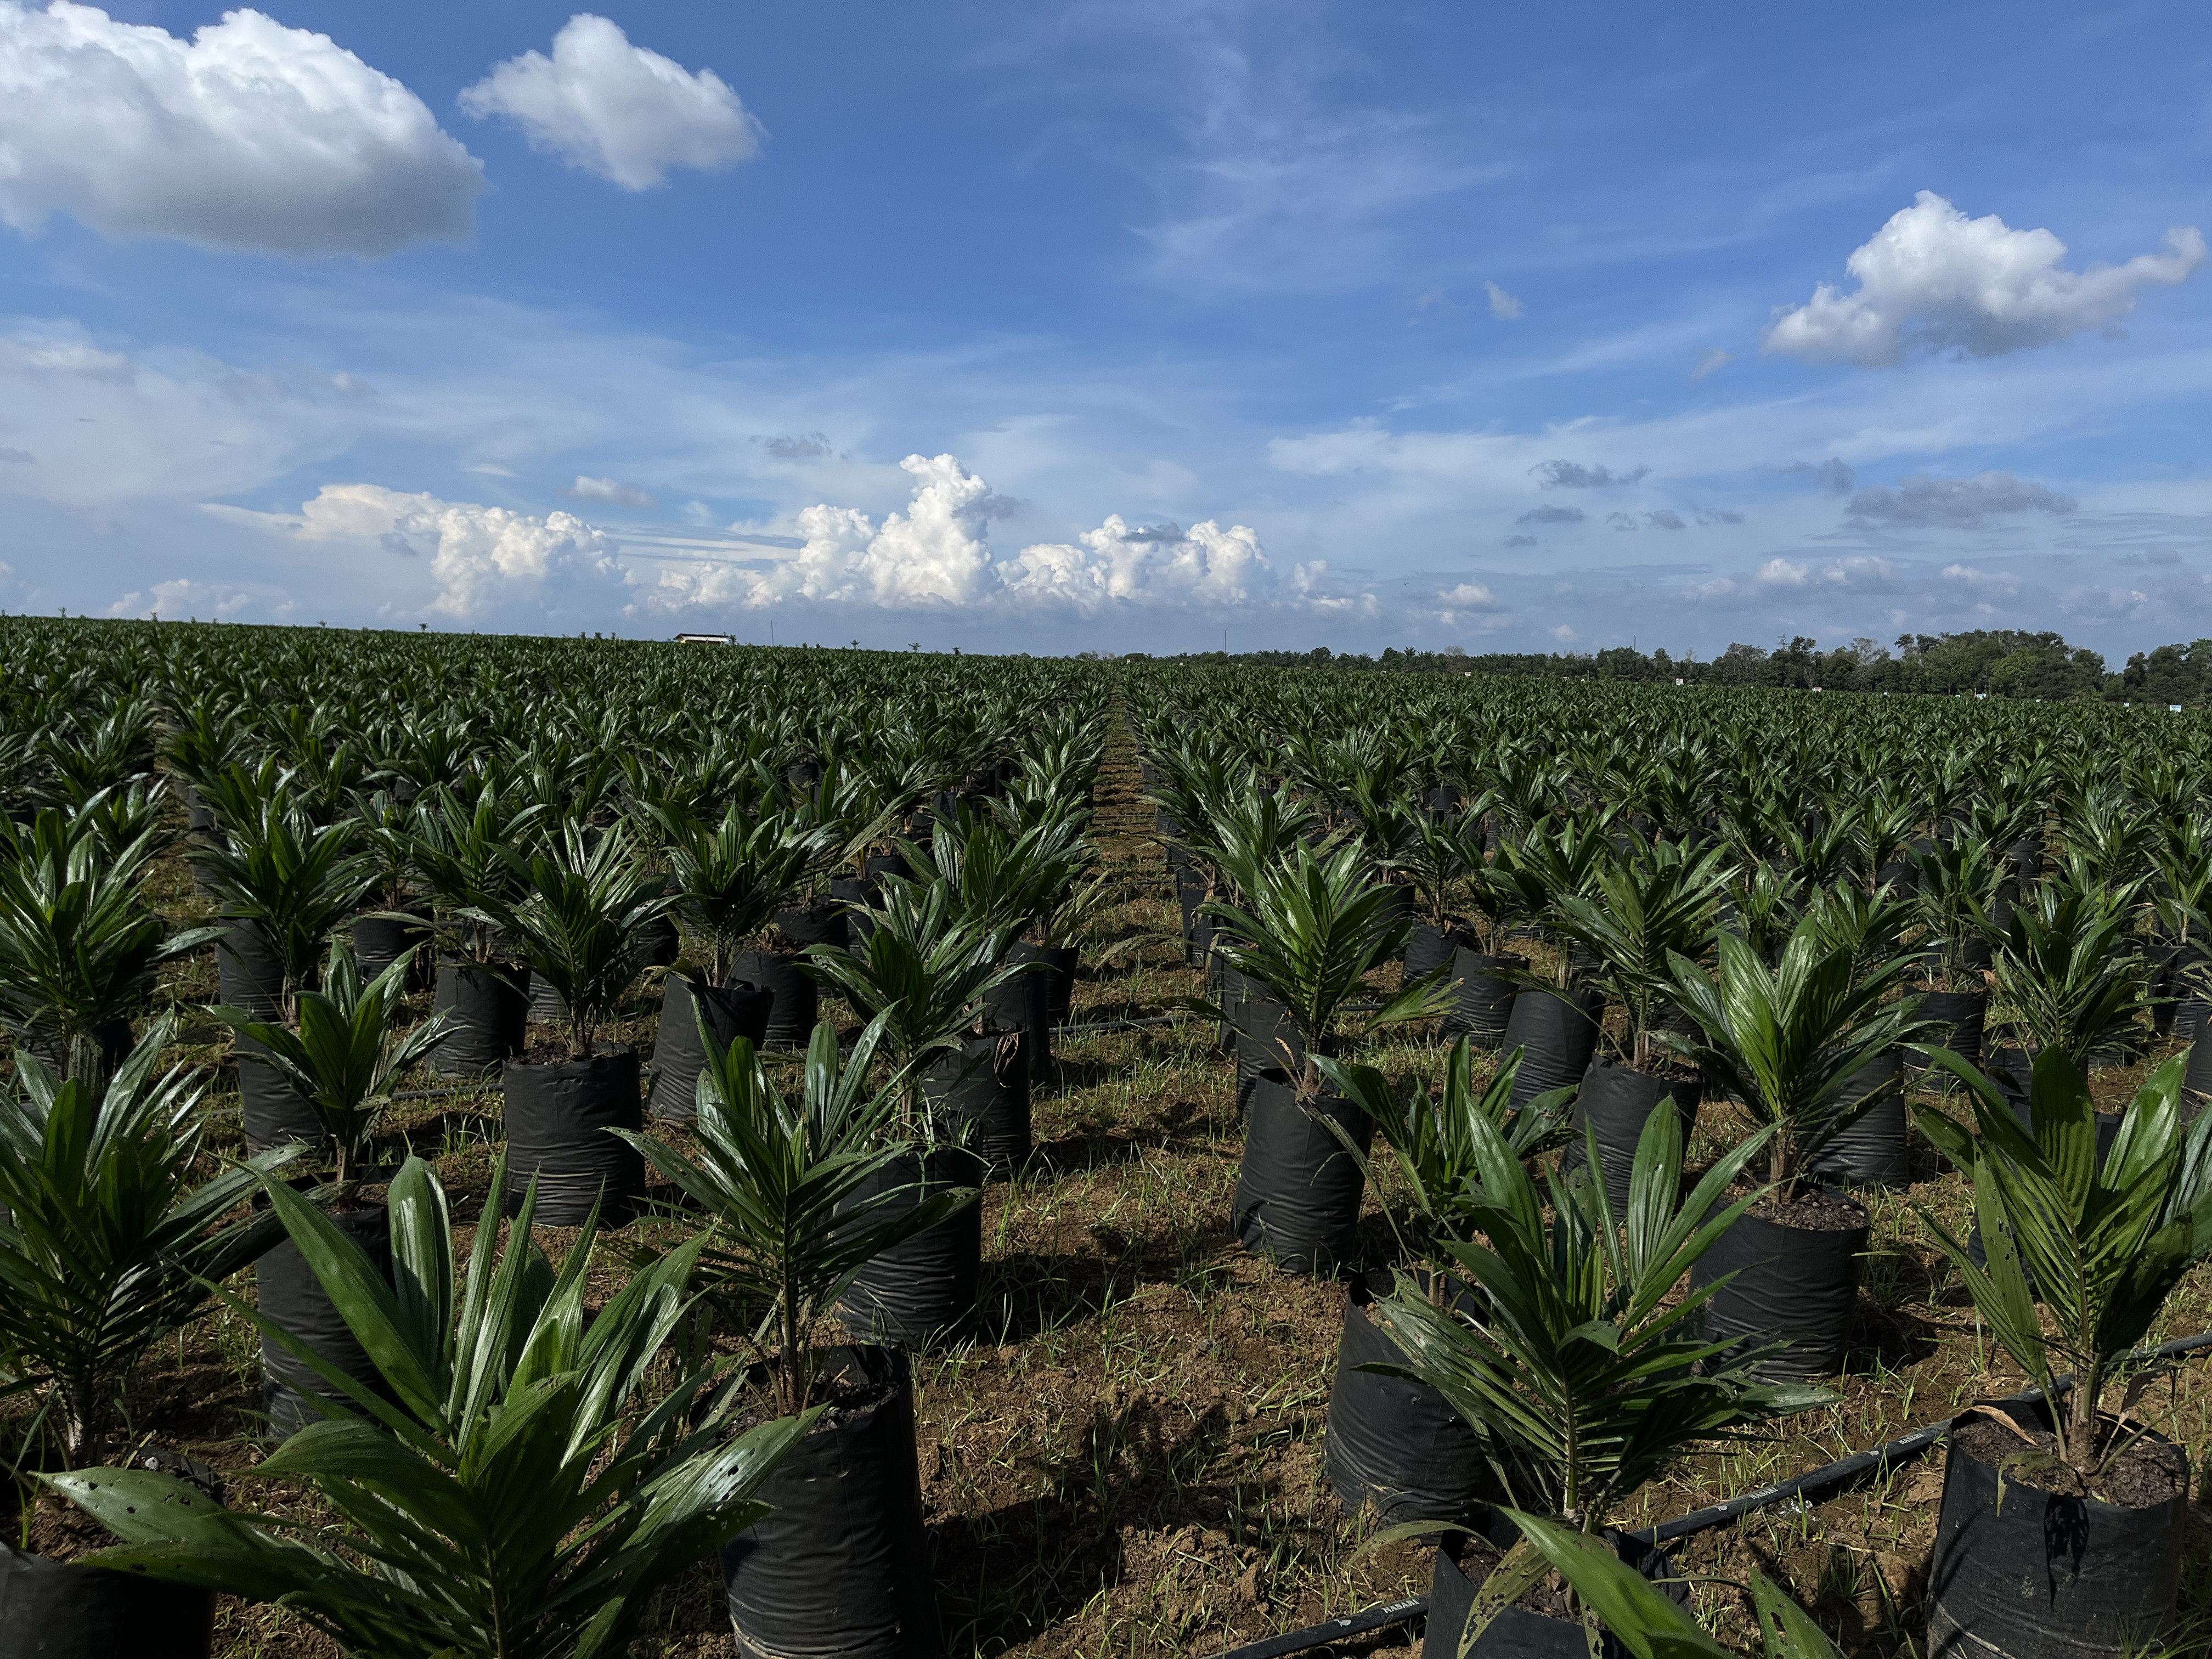
\includegraphics[width=0.5\textwidth]{figure/chapter-2-kelapa-sawit.jpg}
	\caption{\textit{Elaeis Guineensis Jacq} atau Kelapa Sawit}
	\label{fig:2.Kelapa Sawit}
\end{figure}

Seperti terlihat pada Gambar~\ref{fig:2.Kelapa Sawit}, \textit{Elaeis Guineensis Jacq} nama latin dari Kelapa Sawit, merupakan salah satu komoditas perkebunan terpenting di Indonesia. Indonesia adalah produsen dan eksportir minyak kelapa sawit (\textit{Crude Palm Oil}) terbesar di dunia, dengan kontribusi lebih dari 50\% produksi global \cite{abdullah2024potensi}\cite{rejeki2023analisis}. Perkebunan kelapa sawit tersebar luas di Sumatera, Kalimantan, Sulawesi, dan Papua, dengan luas lahan mencapai lebih dari 16 juta hektar pada tahun 2017 \cite{puspitawati2024analisis}.

Industri kelapa sawit memberikan kontribusi signifikan terhadap perekonomian nasional, menyerap jutaan tenaga kerja, serta menjadi sumber devisa utama negara. Selain minyak goreng, produk turunan kelapa sawit juga digunakan dalam industri makanan, kosmetik, farmasi, hingga energi terbarukan (biodiesel) \cite{christian2019industri}. Namun, pengembangan kelapa sawit juga menghadapi tantangan seperti isu lingkungan, deforestasi, dan keberlanjutan yang terus menjadi perhatian nasional maupun internasional.

Di Provinsi Lampung, perkebunan kelapa sawit juga berkembang pesat dan menjadi salah satu komoditas unggulan daerah. Menurut data, luas areal perkebunan kelapa sawit di Lampung tersebar di beberapa kabupaten, seperti Kabupaten Mesuji, Tulang Bawang, Lampung Tengah \cite{kurniasih2021sistem}. Perkebunan ini dikelola oleh perusahaan besar swasta, perkebunan negara, serta petani rakyat. Selain berkontribusi pada perekonomian daerah, pengembangan kelapa sawit di Lampung juga menghadapi tantangan terkait produktivitas, akses pasar, dan isu lingkungan \cite{muflihani2024analisis}.

Selain tantangan terkait produktivitas dan lingkungan, penyakit pada daun bibit kelapa sawit juga menjadi permasalahan penting yang dapat menghambat pertumbuhan dan perkembangan tanaman, terutama pada fase awal pertumbuhan, sekitar 1 minggu hingga 3 bulan awal. Terdapat lima jenis penyakit yang umum menyerang daun bibit kelapa sawit, yaitu bercak daun, daun berputar, daun berkerut, daun menguning, dan daun menggulung.

\subsubsection{Bercak Daun} \label{II.Bercak Daun}
Bercak daun adalah penyakit yang disebabkan oleh jamur patogen dari genus
\textit{Curvularia sp.} merupakan jamur patogen utama penyebab penyakit bercak daun pada bibit kelapa sawit \cite{lalang2016inventarisasi}\cite{suhesti2022analisis}. Infeksi jamur ini ditandai dengan munculnya bercak kecil berwarna kuning hingga coklat pada permukaan daun, yang secara progresif meluas dan menyebabkan nekrosis jaringan. Bercak biasanya berbentuk oval atau tidak beraturan, sering kali dikelilingi warna kuning dan pada serangan berat dapat menyebabkan daun mengering serta gugur sebelum waktunya \cite{agustina2019rapid}. Penyakit ini dapat dilihat pada Gambar \ref{fig:2.Bercak Daun}.

\begin{figure}[H]
	\centering
	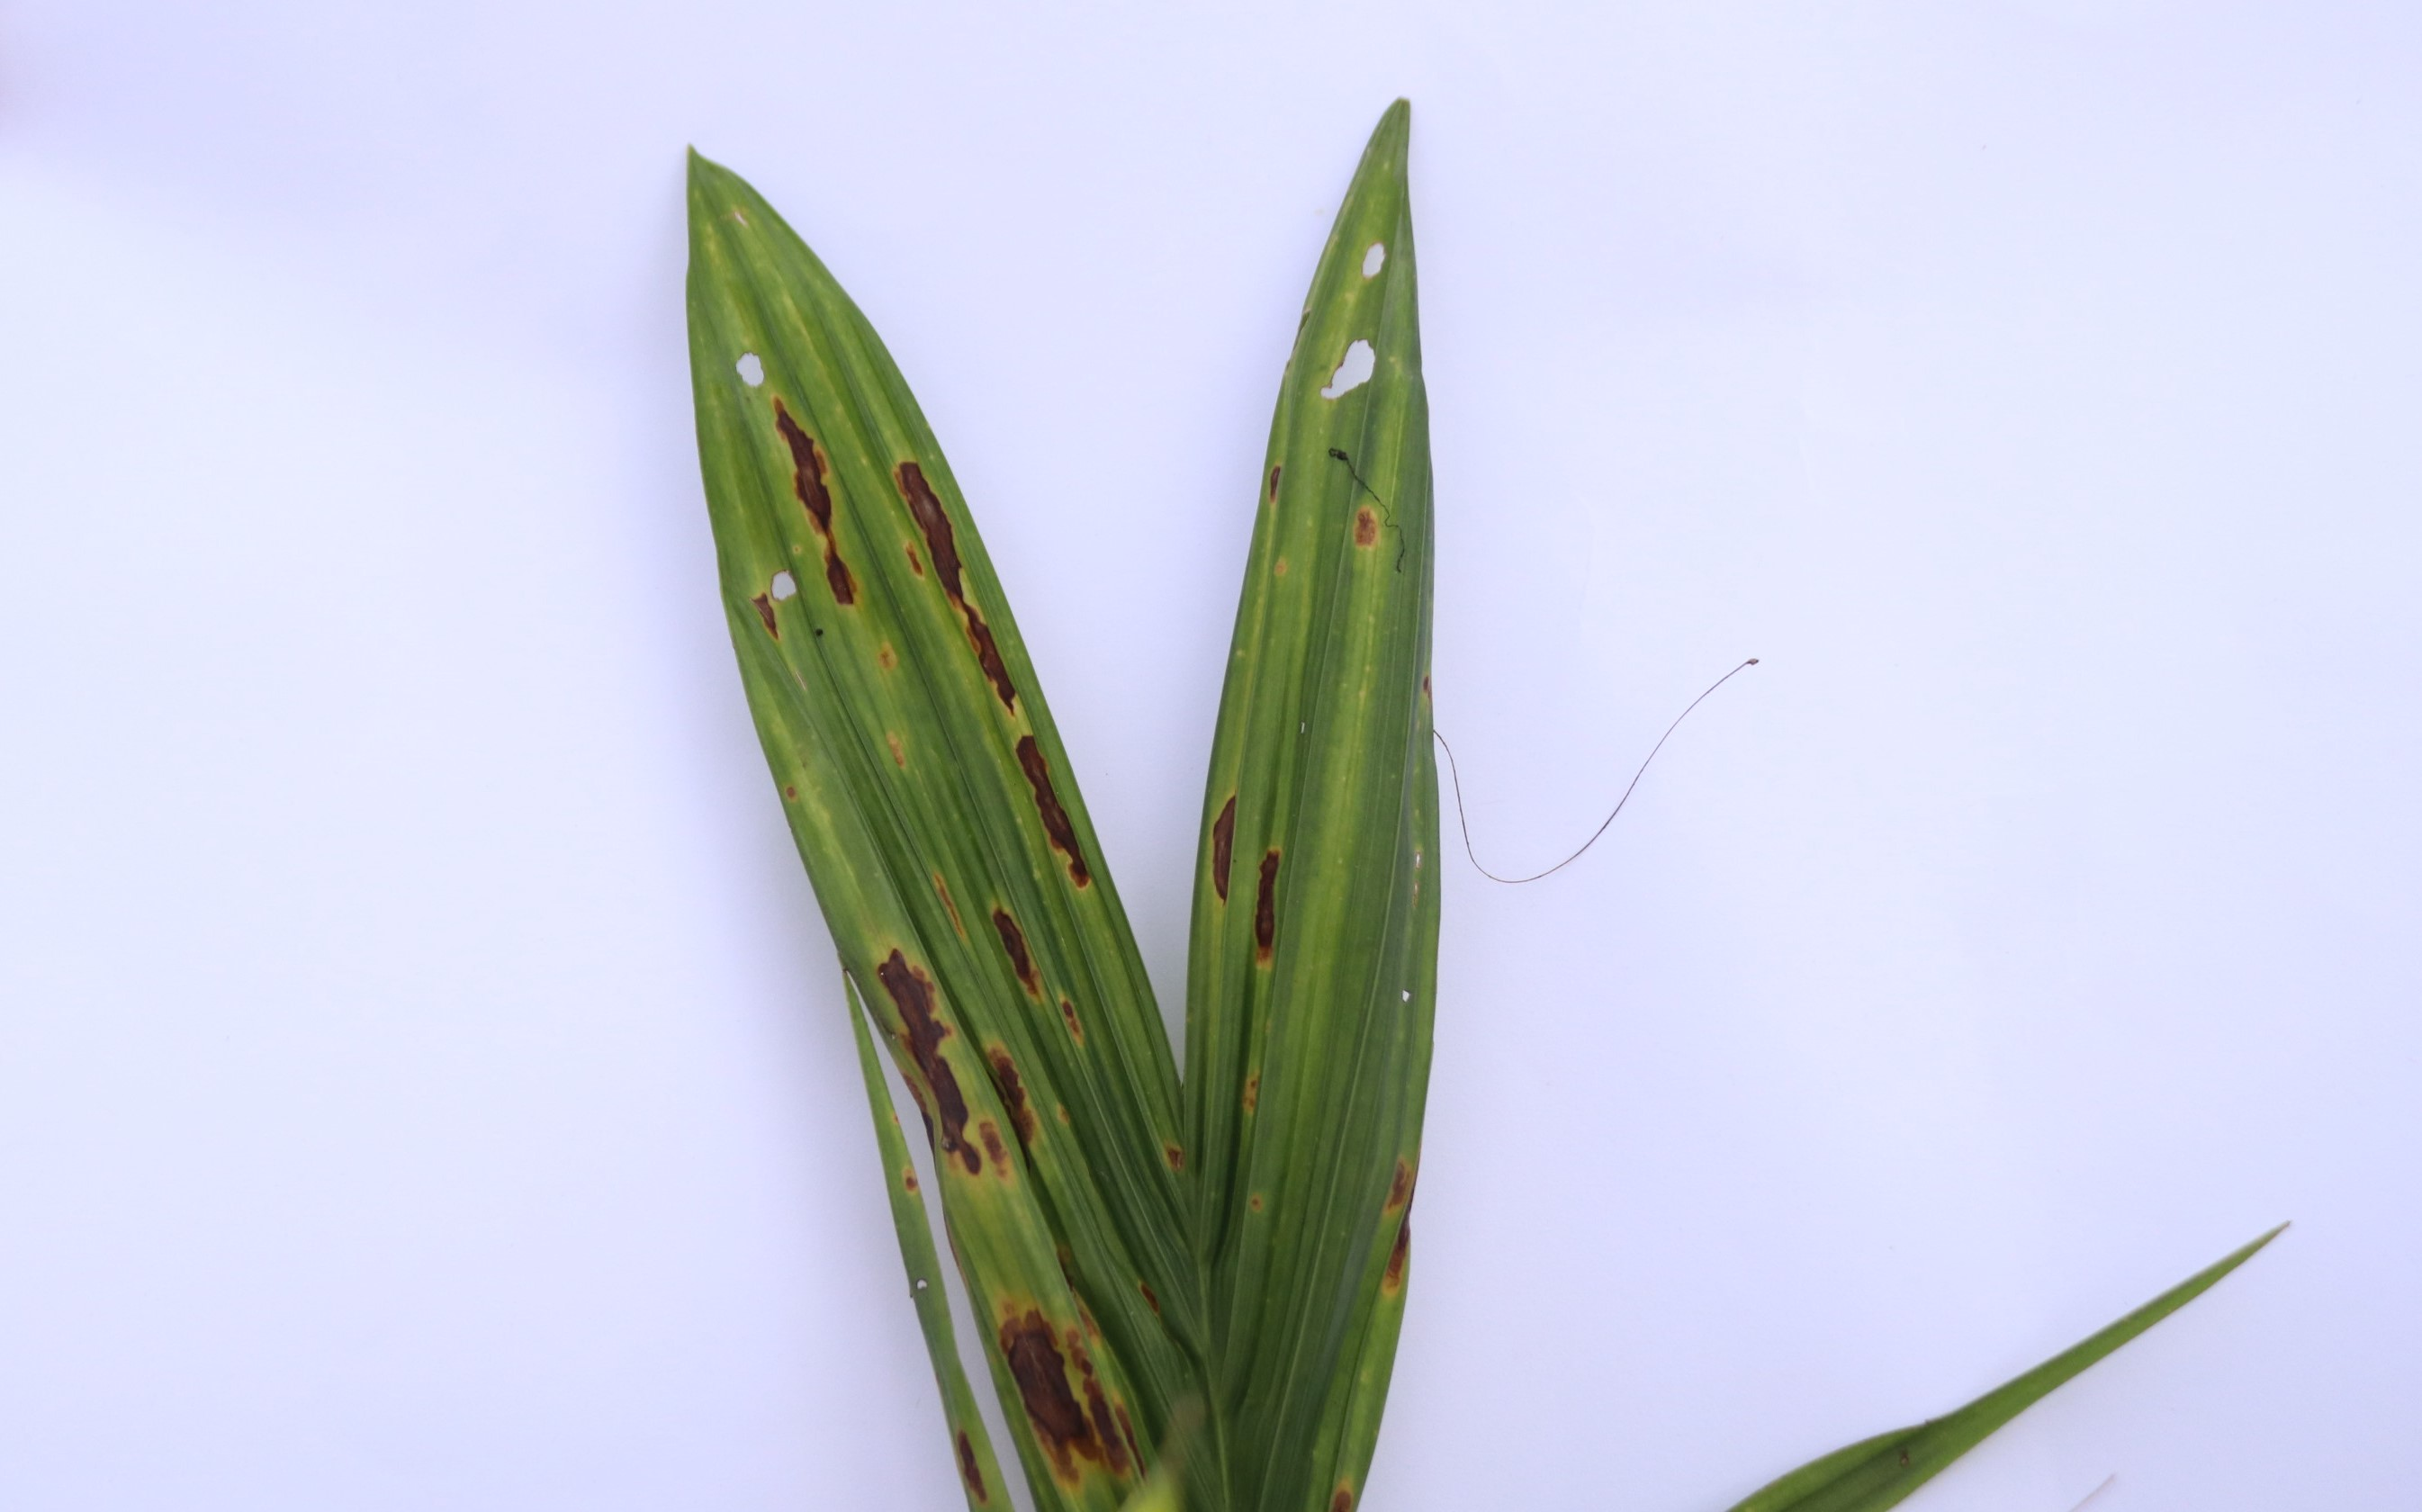
\includegraphics[width=0.5\textwidth]{figure/chapter-2-bercak-daun.jpg}
	\caption{Bercak Daun}
	\label{fig:2.Bercak Daun}
\end{figure}

Penyakit ini dapat berdampak langsung pada penurunan kapasitas fotosintesis akibat rusaknya jaringan daun, sehingga pertumbuhan bibit menjadi terhambat dan produktivitas tanaman dewasa berkurang. Penyebaran \textit{Curvularia sp.} dapat melalui angin, percikan air hujan dan alat pertanian yang terkontaminasi, terutama pada kondisi lingkungan lembap dan sirkulasi udara yang buruk \cite{agustina2019rapid}.

\subsubsection{Daun Berputar} \label{II.Daun Berputar}
Daun berputar adalah penyakit yang disebabkan oleh infeksi virus dan faktor genetik. Penyakit ini ditandai dengan daun yang tumbuh melingkar atau berputar, serta pertumbuhan yang terhambat. Gejala awal biasanya muncul pada daun muda, di mana daun tampak lebih kecil dari ukuran normal dan memiliki bentuk yang tidak simetris. Pada serangan berat, daun dapat mengalami deformasi parah dan menguning, serta pertumbuhan tanaman menjadi terhambat \cite{afriliya2019keanekaragaman}\cite{suhesti2022analisis}. Penyakit ini dapat dilihat pada Gambar \ref{fig:2.Daun Berputar}.

\begin{figure}[H]
	\centering
	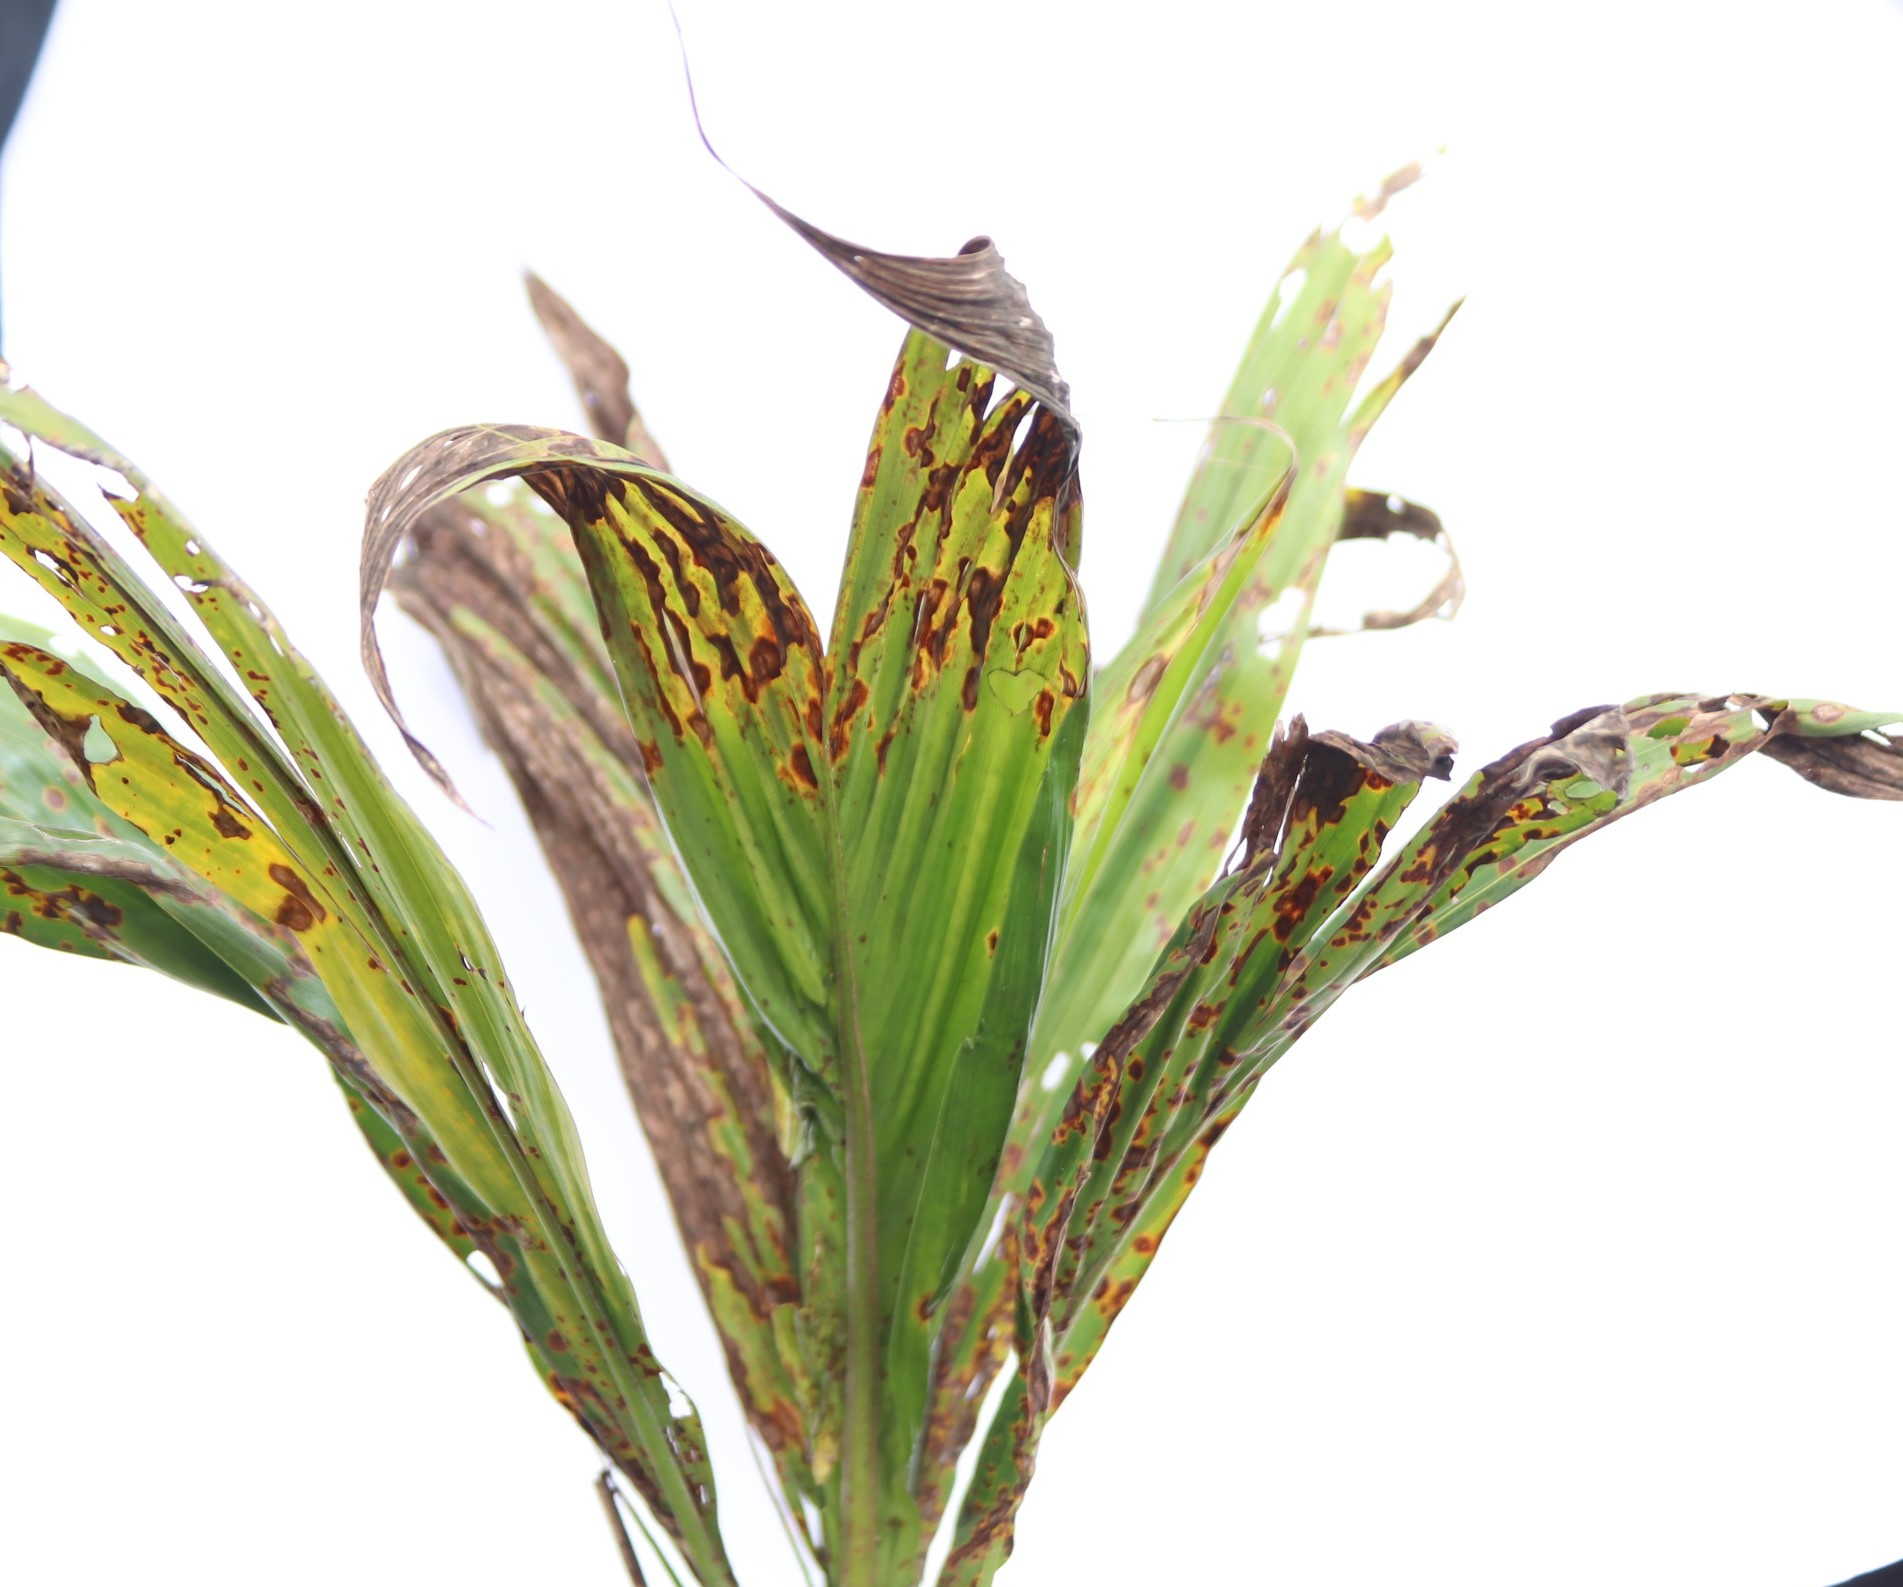
\includegraphics[width=0.5\textwidth]{figure/chapter-2-daun-berputar.jpg}
	\caption{Daun Berputar}
	\label{fig:2.Daun Berputar}
\end{figure}

Penyakit ini dapat menyebar melalui faktor serangga kutu daun dan melalui alat pertanian yang terkontaminasi. Lingkungan yang lembap dan suhu tinggi juga dapat meningkatkan risiko infeksi. Daun berputar dapat menyebabkan penurunan hasil panen pada tanaman dewasa, sehingga penting untuk melakukan pengendalian secara dini \cite{malado2024pengendalian}.

\subsubsection{Daun Berkerut} \label{II.Daun Berkerut}
Daun berkerut pada bibit kelapa sawit merupakan kondisi fisiologis di mana permukaan daun tampak mengerut, tidak rata dan sering kali melipat secara tidak beraturan. Penyakit ini umumnya disebabkan oleh ketidakseimbangan suplai air dan unsur hara mikro, terutama pada masa pertumbuhan awal bibit \cite{rahayu2023penyakit}\cite{suhesti2022analisis}. Faktor lingkungan seperti kelembapan rendah, paparan sinar matahari yang minim atau terlalu berlebihan, serta media tanam yang kurang optimal dapat memperparah gejala ini \cite{syahfari2024buku}. Penyakit ini dapat dilihat pada Gambar \ref{fig:2.Daun Berkerut}.

\begin{figure}[H]
	\centering
	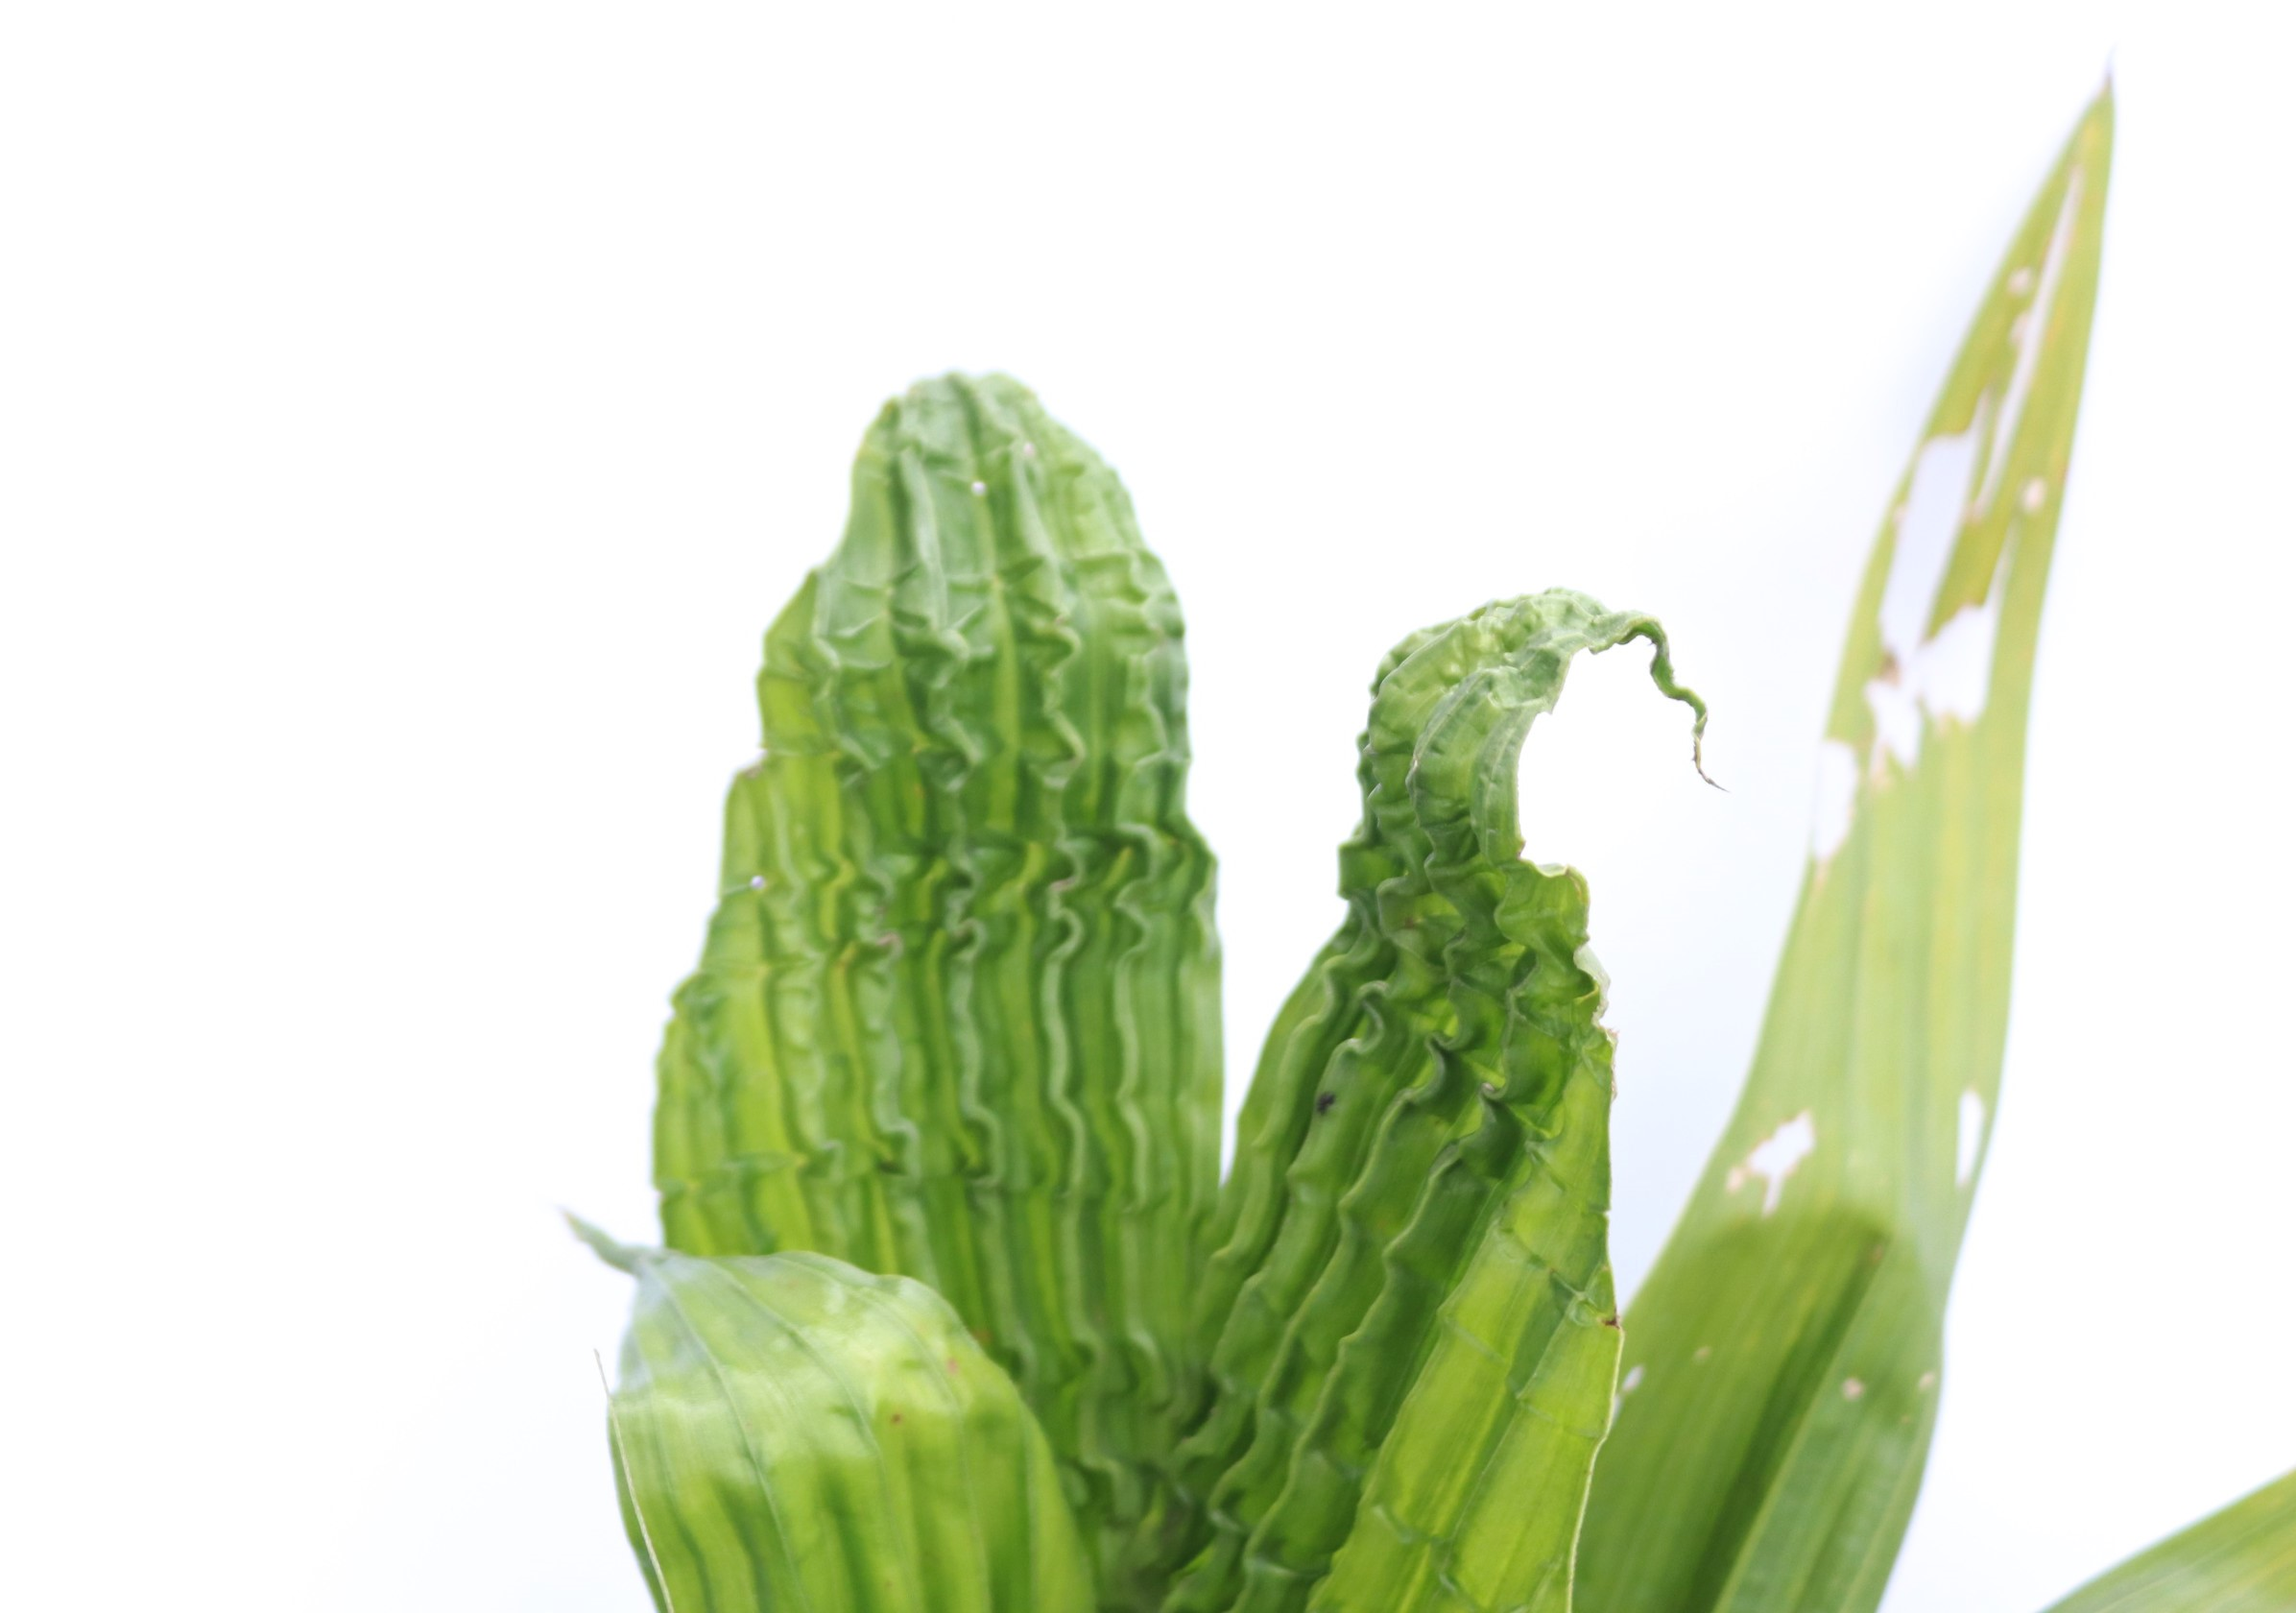
\includegraphics[width=0.5\textwidth]{figure/chapter-2-daun-berkerut.jpg}
	\caption{Daun Berkerut}
	\label{fig:2.Daun Berkerut}
\end{figure}

Daun berkerut dapat mengganggu proses fotosintesis dan penyerapan cahaya, sehingga menghambat pertumbuhan bibit. Gejala awal biasanya muncul pada daun muda, di mana daun tampak lebih kecil dari ukuran normal dan memiliki bentuk yang tidak simetris. Pada serangan berat, daun dapat mengalami deformasi parah dan menguning, serta pertumbuhan tanaman menjadi terhambat.  

\subsubsection{Daun Menguning} \label{II.Daun Menguning}
Daun menguning adalah penyakit yang ditandai dengan perubahan warna daun dari hijau menjadi kuning, yang dapat disebabkan oleh berbagai faktor, termasuk kekurangan unsur hara, serangan hama, infeksi patogen, dan kondisi lingkungan yang tidak optimal \cite{afriliya2019keanekaragaman}\cite{suhesti2022analisis}. Penyakit ini dapat dilihat pada Gambar \ref{fig:2.Daun Menguning}.

\begin{figure}[H]
	\centering
	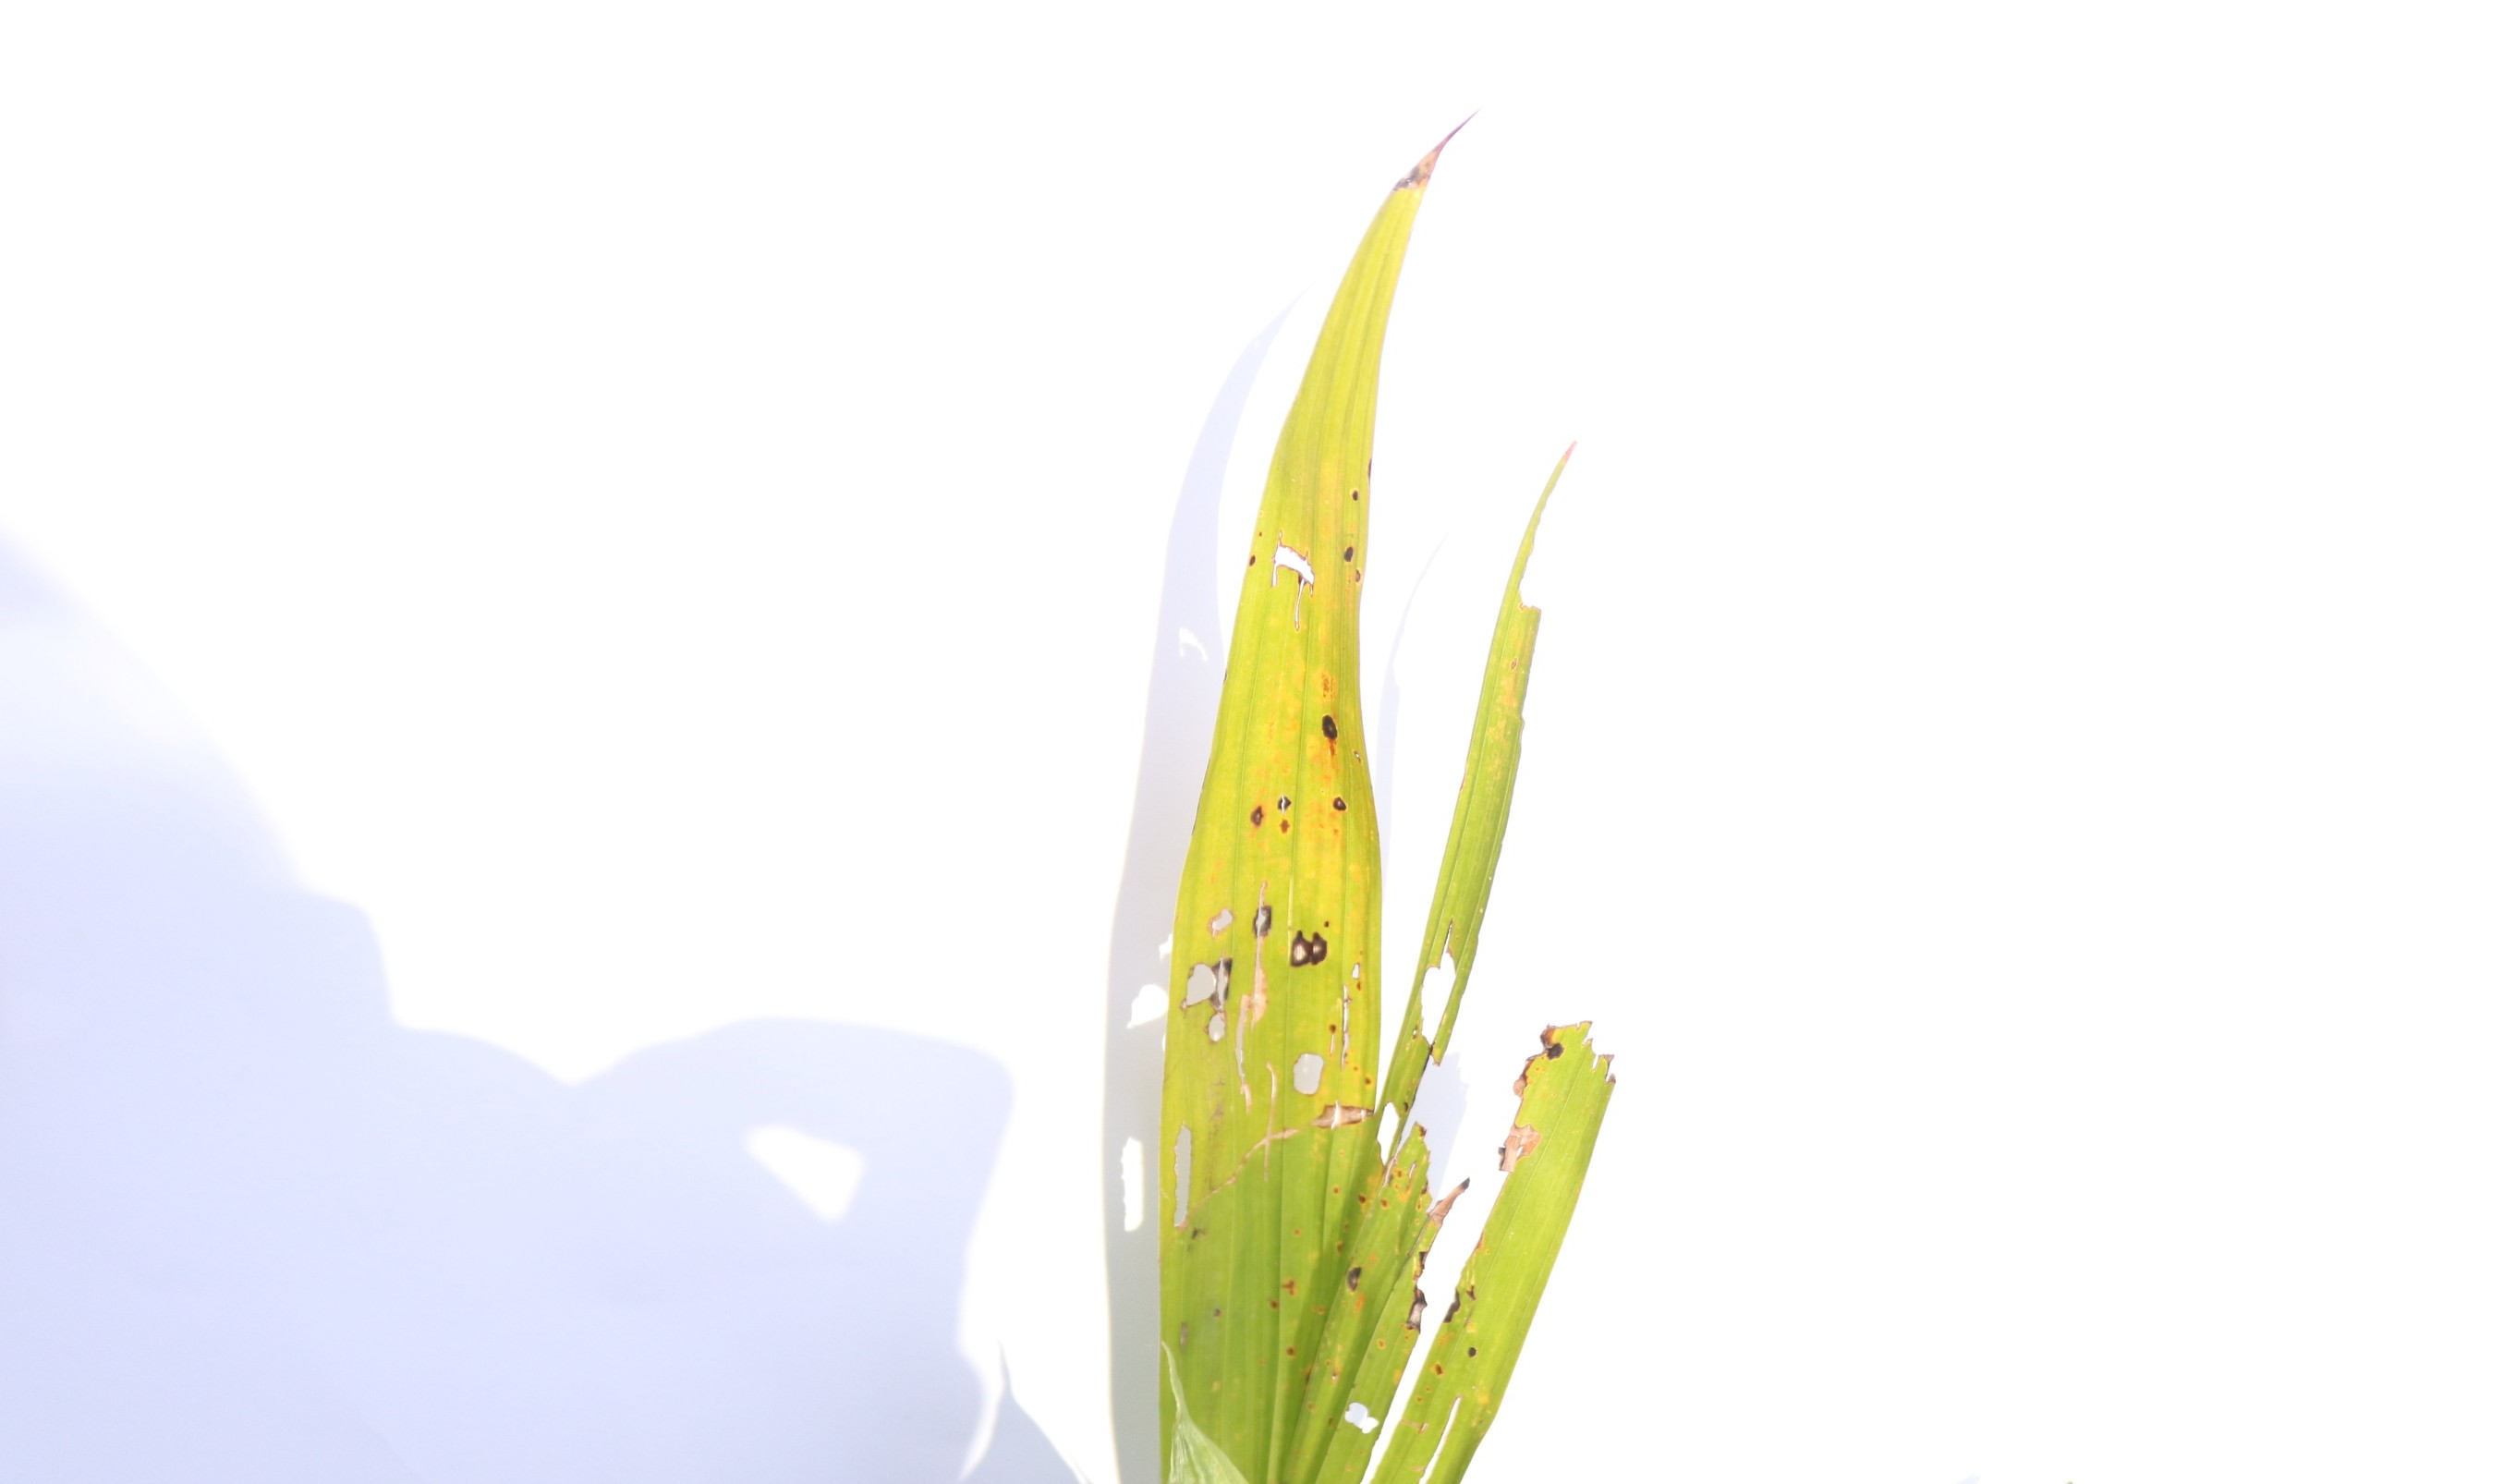
\includegraphics[width=0.5\textwidth]{figure/chapter-2-daun-menguning.jpg}
	\caption{Daun Menguning}
	\label{fig:2.Daun Menguning}
\end{figure}

Penyakit juga dapat disebabkan oleh kekurangan unsur hara, seperti nitrogen, fosfor, dan kalium, yang berperan penting dalam proses fotosintesis dan pertumbuhan tanaman. Selain itu, serangan hama seperti kutu daun dan ulat juga dapat menyebabkan daun menguning \cite{suhesti2022analisis}. Lingkungan yang tidak optimal, seperti suhu ekstrem atau kelembapan yang rendah, juga dapat memicu gejala ini. 

\subsubsection{Daun Menggulung} \label{II.Daun Menggulung}
Daun menggulung adalah penyakit yang ditandai dengan perubahan bentuk daun yang melipat atau menggulung ke arah dalam, sehingga mengurangi luas permukaan daun yang dapat menyerap cahaya matahari. Penyakit ini dapat disebabkan oleh infeksi virus, serangan hama, atau faktor lingkungan yang tidak optimal \cite{hanik2024identification}\cite{suhesti2022analisis}. Penyakit ini dapat dilihat pada Gambar \ref{fig:2.Daun Menggulung}.

\begin{figure}[H]
	\centering
	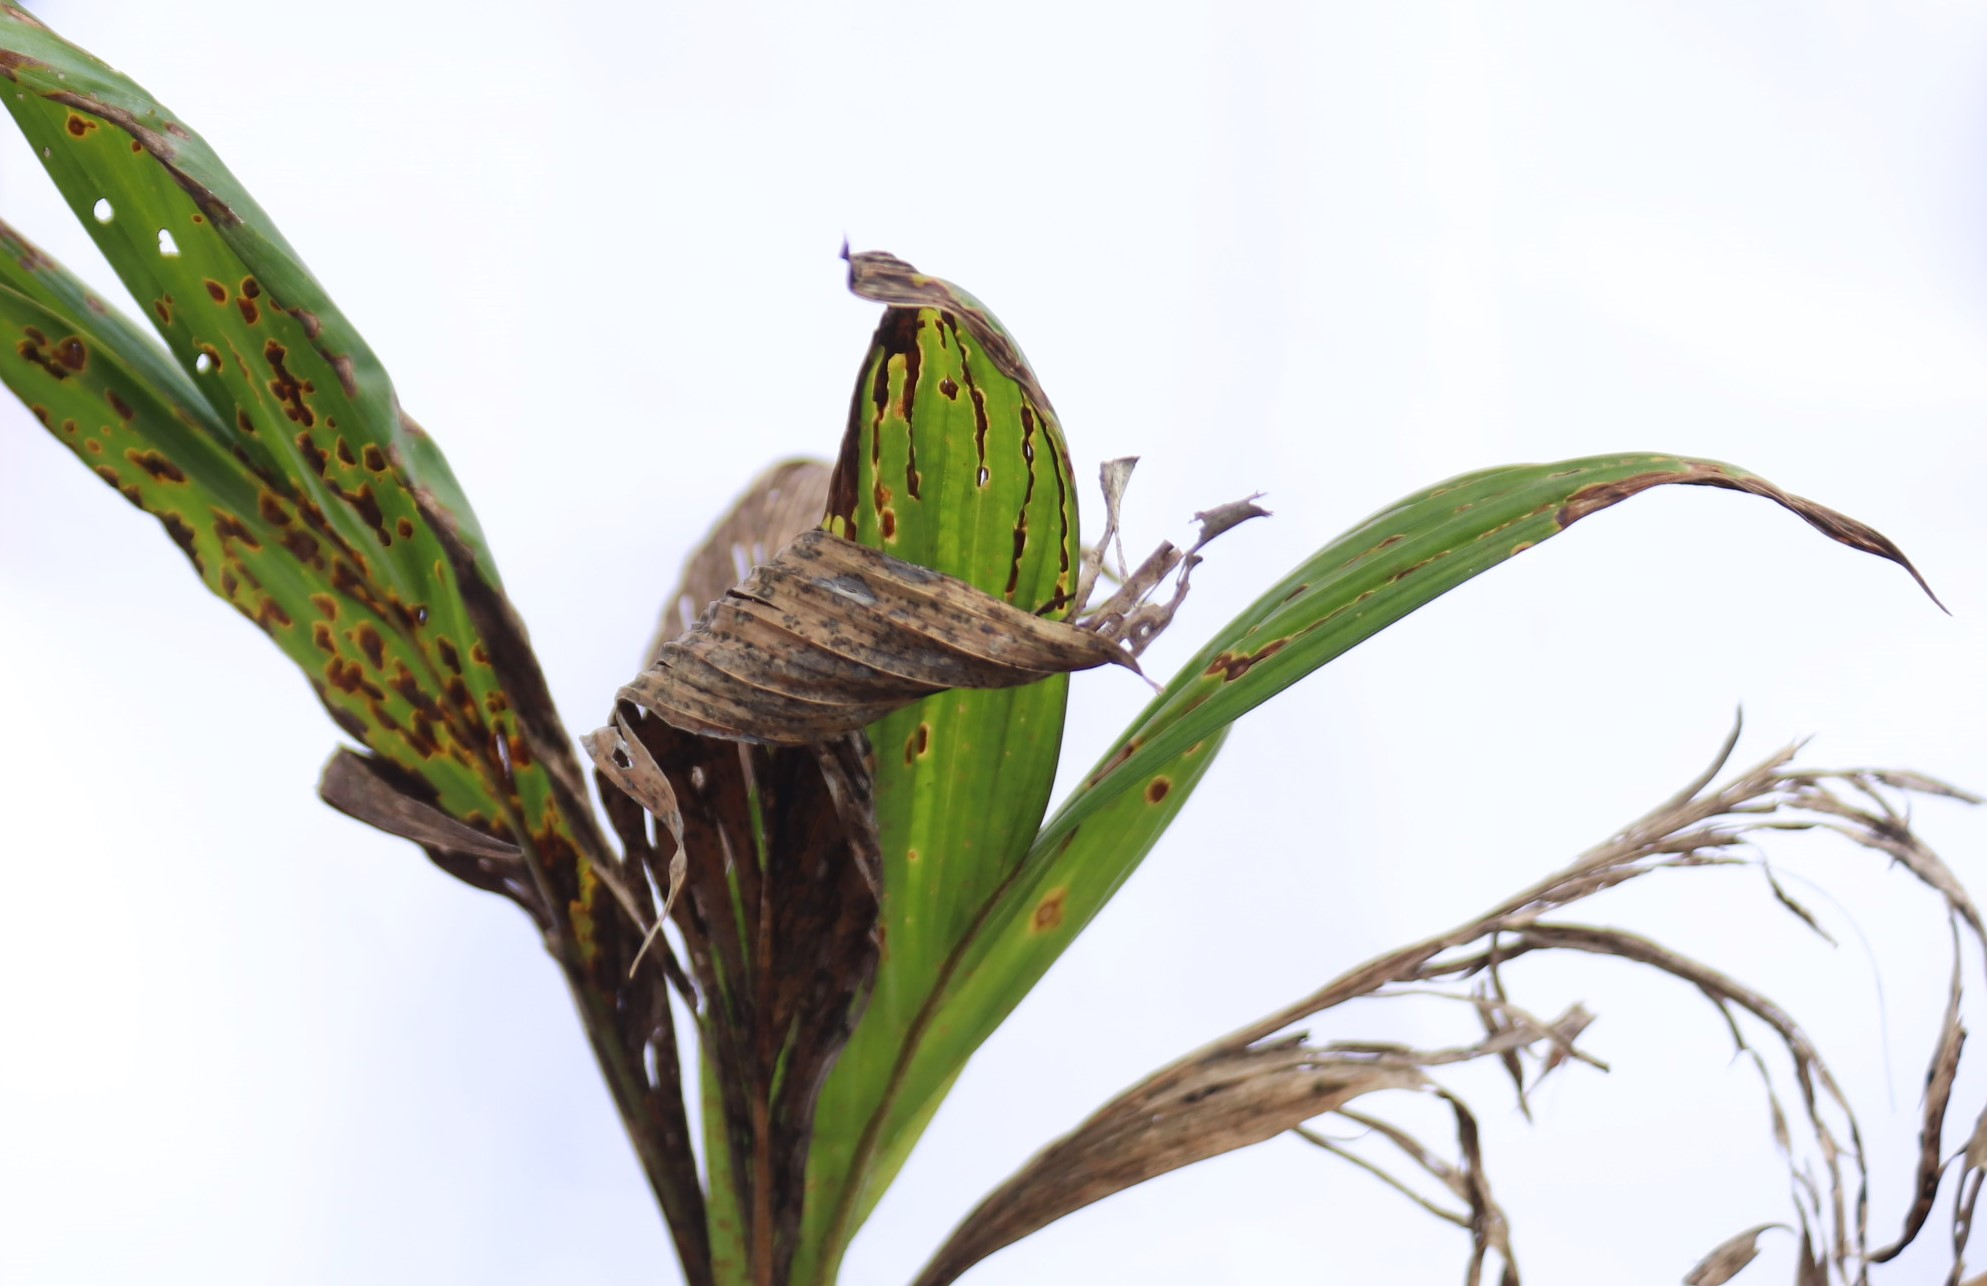
\includegraphics[width=0.5\textwidth]{figure/chapter-2-daun-menggulung.jpg}
	\caption{Daun Menggulung}
	\label{fig:2.Daun Menggulung}
\end{figure}

Penyakit ini dapat disebabkan oleh infeksi virus, melalui hama serangga, seperti kutu daun dan ulat \cite{suhesti2022analisis}. Lingkungan yang tidak optimal, seperti suhu ekstrem atau kelembapan yang rendah, juga dapat memicu gejala ini. Jika tidak segera ditangani, daun menggulung dapat mengganggu proses fotosintesis dan mengurangi hasil panen.
% --------------
\subsection{\textit{Naïve Bayes}}\label{II.NaiveBayes}

\textit{Naïve Bayes} merupakan salah satu metode klasifikasi berbasis probabilistik yang paling sederhana dan efisien, serta banyak digunakan dalam berbagai kasus klasifikasi seperti pengenalan citra, analisis teks, dan deteksi penyakit. Metode ini didasarkan pada Teorema Bayes dengan asumsi bahwa setiap fitur (atribut) pada data bersifat saling bebas (independen) \cite{aziz2024analisis}.

Dalam konteks klasifikasi, \textit{Naïve Bayes} bertujuan untuk menentukan kelas $C_k$ yang paling mungkin diberikan fitur-fitur $X = (x_1, x_2, ..., x_n)$ dari suatu data. Proses klasifikasi dilakukan dengan menghitung probabilitas posterior menggunakan Teorema Bayes sebagai berikut:
\begin{equation}
	P(C_k|X) = \frac{P(X|C_k) \cdot P(C_k)}{P(X)}
	\label{eq:naive_bayes}
\end{equation}
\myequations{Persamaan Klasifikasi \textit{Naïve Bayes}}

\vspace{0.5em}

\noindent
Dengan keterangan sebagai berikut:\\[0.5em]
\hspace*{1.5em}$P(C_k|X)$ : probabilitas kelas $C_k$ diberikan fitur $X$ (posterior)\\
\hspace*{1.5em}$P(X|C_k)$ : probabilitas fitur $X$ terjadi jika kelas $C_k$ benar (likelihood)\\
\hspace*{1.5em}$P(C_k)$ \hspace{0.65em}: probabilitas awal kelas $C_k$ (prior)\\
\hspace*{1.5em}$P(X)$ \hspace{0.65em}: probabilitas total fitur $X$ (evidence)	

Dalam prakteknya, karena $P(X)$ adalah konstan untuk semua kelas, maka proses klasifikasi dapat disederhanakan menjadi:
\begin{equation}
	\hat{C} = \arg\max_{C_k} \; P(C_k) \cdot P(X|C_k)
\end{equation}	
\myequations{Persamaan Klasifikasi Sederhana \textit{Naïve Bayes}}

\noindent
Dimana $\hat{C}$ adalah kelas yang diprediksi.

Jika fitur $X = (x_1, x_2, ..., x_n)$ dianggap independen, maka:
\begin{equation}
	P(X|C_k) = \prod_{i=1}^{n} P(x_i | C_k)
\end{equation}
\myequations{Persamaan Independen Fitur \textit{Naïve Bayes}}

\noindent
Dengan keterangan sebagai berikut:\\[0.5em]
\hspace*{1.5em}$P(X|C_k)$ : probabilitas fitur $X$ terjadi jika kelasSS $C_k$ benar (likelihood)\\
\hspace*{1.5em}$P(x_i|C_k)$ : probabilitas fitur ke-$i$ terjadi jika kelas $C_k$ benar (likelihood)\\


% --------------
\subsubsection{Teorema Bayes}\label{II.Teorema Bayes}
Teorema Bayes adalah prinsip dasar yang digunakan dalam \textit{Naïve Bayes} untuk menghitung probabilitas posterior dari suatu hipotesis berdasarkan data yang diamati \cite{watratan2020implementasi}. Teorema ini menyatakan bahwa probabilitas suatu hipotesis $H$ diberikan data $X$ dapat dihitung dengan menggunakan probabilitas awal $P(H)$, probabilitas data $X$ diberikan hipotesis $H$ dan probabilitas total data $X$ \cite{Muhamad2017OptimasiNB}.

Persamaan umum dari Teorema Bayes dinyatakan sebagai berikut:
\begin{equation}
	P(H|X) = \frac{P(X|H) \cdot P(H)}{P(X)}
	\label{eq:bayes}
\end{equation}
\myequations{Persamaan Teorema Bayes}

\vspace{0.5em}

\noindent
Dengan keterangan sebagai berikut:\\[0.5em]
\hspace*{1.5em}$P(H|X)$ : probabilitas hipotesis $H$ diberikan data $X$ (posterior)\\
\hspace*{1.5em}$P(X|H)$ : probabilitas data $X$ terjadi jika $H$ benar (likelihood)\\
\hspace*{1.5em}$P(H)$ \hspace{0.65em}: probabilitas awal hipotesis $H$ (prior)\\
\hspace*{1.5em}$P(X)$ \hspace{0.65em}: probabilitas total data $X$ (evidence)

% Tujuan utama dari klasifikasi menggunakan \textit{Naïve Bayes} adalah memilih kelas $C_k$ yang memaksimalkan nilai posterior $P(C_k|X)$, sehingga proses klasifikasi dapat ditulis sebagai:

% \begin{equation}
% \hat{C} = \arg\max_{C_k} P(C_k|X)
% \end{equation}

% Berdasarkan Teorema Bayes, karena nilai $P(X)$ konstan untuk semua kelas, maka cukup dihitung:
% \begin{equation}
% \hat{C} = \arg\max_{C_k} \; P(C_k) \cdot P(X|C_k)
% \end{equation}

% Jika fitur $X = (x_1, x_2, ..., x_n)$ dianggap independen, maka:
% \begin{equation}
% P(X|C_k) = \prod_{i=1}^{n} P(x_i | C_k)
% \end{equation}

\subsubsection{Distribusi Gaussian Fitur Numerik}\label{II.Distribusi Gaussian Fitur Numerik}
\textit{Naïve Bayes} dapat digunakan untuk data numerik dengan asumsi bahwa fitur-fitur tersebut mengikuti distribusi Gaussian. Dalam hal ini, kita perlu menghitung probabilitas dari setiap fitur $x_i$ pada kelas $C_k$ menggunakan distribusi normal (Gaussian) \cite{Riza2025KlasifikasiVK}.
Untuk fitur numerik yang diasumsikan mengikuti distribusi normal (Gaussian), nilai probabilitas dihitung dengan:

\begin{equation}
	P(x_i | C_k) = \frac{1}{\sqrt{2\pi\sigma_{k,i}^2}} \exp \left( -\frac{(x_i - \mu_{k,i})^2}{2\sigma_{k,i}^2} \right)
	\label{eq:gaussian}
\end{equation}
\myequations{Nilai Probabilitas Ditribusi Normal}

% \noindent
% dengan:
% \begin{itemize}
%     \item $\mu_{k,i}$ : rata-rata fitur ke-$i$ pada kelas $C_k$
%     \item $\sigma_{k,i}$ : standar deviasi fitur ke-$i$ pada kelas $C_k$
% \end{itemize}

\noindent
Dengan keterangan sebagai berikut:\\[0.5em]
\hspace*{1.5em}$\mu_{k,i}$ \hspace{0.4em}: rata-rata fitur ke-$i$ pada kelas $C_k$\\
\hspace*{1.5em}$\sigma_{k,i}$ : standar deviasi fitur ke-$i$ pada kelas $C_k$

Pada data bertipe numerik, proses perhitungannya memiliki beberapa tahapan khusus yang berbeda dari persamaan umum sebelumnya. Langkah-langkah yang dilakukan adalah sebagai berikut:

\begin{enumerate}
	\item \textbf{Menghitung nilai rata-rata (mean)} untuk setiap fitur:
			\begin{equation}
				\mu = \frac{1}{n} \sum_{i=1}^{n} x_i
				\label{eq:mean}
			\end{equation}
			\myequations{Nilai Rata-rata (mean)}
		Dengan keterangan sebagai berikut:\\[0.5em]
		\hspace*{1.5em}$\mu$ : rata-rata fitur\\
		\hspace*{1.5em}$x_i$ : nilai fitur ke-$i$\\
		\hspace*{1.5em}$n$ : jumlah data pada kelas tertentu

		\item \textbf{Menghitung standar deviasi ($\sigma$)}:
			\begin{equation}
				\sigma = \sqrt{ \frac{1}{n} \sum_{i=1}^{n} (x_i - \mu)^2 }
				\label{eq:stddev}
			\end{equation}
			\myequations{Nilai Standar Deviasi ($\sigma$)}
			Dengan keterangan sebagai berikut:\\[0.5em]
			\hspace*{1.5em}$\sigma$ : standar deviasi fitur\\
			\hspace*{1.5em}$x_i$ : nilai fitur ke-$i$\\
			\hspace*{1.5em}$\mu$ : rata-rata fitur\\
			\hspace*{1.5em}$n$ : jumlah data pada kelas tertentu

		\item \textbf{Menghitung likelihood} menggunakan distribusi Gaussian berdasarkan persamaan~\eqref{eq:gaussian}.\\
		Likelihood adalah probabilitas kemunculan data fitur $x_i$ pada kelas $C_k$, yaitu $P(x_i|C_k)$, yang menunjukkan seberapa besar kemungkinan data tersebut muncul jika diketahui kelasnya.

		\item \textbf{Menghitung probabilitas posterior} untuk setiap kelas:
	
		Probabilitas posterior adalah probabilitas suatu kelas $C_k$ setelah mempertimbangkan data fitur $X$ yang diamati. Nilai ini dihitung dengan mengalikan probabilitas awal (prior) kelas $C_k$ dengan hasil perkalian probabilitas setiap fitur $x_i$ pada kelas tersebut, sesuai dengan rumus berikut:
		\begin{equation}
			P(C_k|X) \propto P(C_k) \cdot \prod_{i=1}^{n} P(x_i | C_k)
		\end{equation}
		\myequations{Nilai Probabilitas Posterior}
		Dengan keterangan sebagai berikut:\\[0.5em]
		\hspace*{1.5em}$P(C_k|X)$ : probabilitas posterior kelas $C_k$ terhadap data $X$\\
		\hspace*{1.5em}$P(C_k)$ : probabilitas awal (prior) kelas $C_k$\\
		\hspace*{1.5em}$P(x_i | C_k)$ : probabilitas fitur $x_i$ pada kelas $C_k$\\
		\hspace*{1.5em}$n$ : jumlah fitur pada data $X$

		\item \textbf{Menentukan kelas hasil klasifikasi}:
		\begin{equation}
			\hat{C} = \arg\max_{C_k} \; P(C_k|X)
		\end{equation}
		\myequations{Nilai Kelas Hasil Klasifikasi}
		Dengan keterangan sebagai berikut:\\[0.5em]
		\hspace*{1.5em}$\hat{C}$ : kelas hasil prediksi (kelas dengan probabilitas tertinggi)\\
		\hspace*{1.5em}$P(C_k|X)$ : probabilitas posterior kelas $C_k$ terhadap data $X$
\end{enumerate}

% -------------------
\subsection{Genetic Algorithm} \label{II.Genetic Algorithm}
\textit{Genetic Algorithm} (GA) adalah metode optimasi yang terinspirasi oleh proses evolusi biologis . GA menggunakan prinsip seleksi alam, di mana individu yang lebih baik memiliki peluang lebih besar untuk bertahan dan berkembang biak \cite{Zahro2020OptimasiRute}.

Dalam konteks klasifikasi, GA dapat digunakan untuk memilih fitur yang paling relevan atau mengoptimalkan parameter model. Kelebihan GA adalah kemampuannya untuk menjelajahi ruang solusi yang besar dan kompleks, serta fleksibilitas dalam mengadaptasi berbagai jenis masalah. Namun, kelemahannya adalah waktu komputasi yang lebih lama dibandingkan metode optimasi lainnya \cite{Transmisi68957}. 

Secara umum, proses utama dalam \textit{Genetic Algorithm} meliputi seleksi, crossover, dan mutasi \cite{saputro2015implementasi}. Berikut adalah rumus-rumus yang digunakan dalam setiap tahap:

\subsubsection{Seleksi (Selection)} \label{II.GA.Selection}
Seleksi adalah tahap dalam Genetic Algorithm (GA) yang bertujuan memilih individu-individu terbaik dari populasi berdasarkan nilai fitness-nya untuk menjadi induk (parent) pada generasi berikutnya. Individu dengan nilai fitness lebih tinggi memiliki peluang lebih besar untuk terpilih, sehingga karakteristik yang baik dapat diwariskan ke generasi selanjutnya. Metode seleksi yang umum digunakan antara lain roulette wheel selection, tournament selection, dan rank selection \cite{naufal2025optimization}.

Pada tahap ini, individu-individu dalam populasi dievaluasi berdasarkan fungsi fitness yang telah ditentukan. Fungsi fitness mengukur seberapa baik individu tersebut dalam menyelesaikan masalah yang dihadapi. Setelah itu, individu-individu dengan nilai fitness tertinggi akan dipilih untuk menjadi induk pada generasi berikutnya \cite{naufal2025optimization}\cite{Matousek2008GeneticAA}.

Sebagai contoh, jika kita memiliki populasi $P = \{I_1, I_2, ..., I_N\}$ dengan nilai fitness masing-masing $f_i$ \cite{Matousek2008GeneticAA}, misalnya menggunakan \textit{Roulette Wheel Selection}, maka kita dapat menghitung probabilitas seleksi untuk setiap individu sebagai berikut:
\begin{equation}
	P_i = \frac{f_i}{\sum_{j=1}^{N} f_j}
	\label{eq:ga-selection}
\end{equation}
\myequations{Nilai Probabilitas Seleksi}
dengan $P_i$ adalah probabilitas individu ke-$i$ terpilih, $f_i$ adalah nilai fitness individu ke-$i$, dan $N$ adalah jumlah total individu dalam populasi.

\vspace{0.5em}

\subsubsection{Crossover} \label{II.GA.Crossover}
Crossover adalah proses pertukaran gen antara dua individu (parent) untuk menghasilkan individu baru (offspring). Proses ini bertujuan untuk menggabungkan informasi genetik dari kedua parent untuk menciptakan individu yang lebih baik. Crossover dapat dilakukan dengan berbagai cara, seperti \textit{Single Point Crossover}, \textit{Two Point Crossover}, atau \textit{Uniform Crossover} \cite{Pachuau2020AnOO}.

Crossover dilakukan dengan memilih dua parent dari populasi yang telah diseleksi, kemudian memilih titik crossover secara acak pada kromosom \cite{Fadhilah2016RepresentasiMU}. Setelah itu, gen-gen di antara kedua parent akan ditukar untuk membentuk dua individu baru (offspring). Proses ini diulang hingga jumlah individu baru yang diinginkan tercapai \cite{Muliantara2013ANALISISDI}.

Sebagai contoh, jika kita memiliki dua parent $P_1 = (g_{1,1}, g_{1,2}, ..., g_{1,n})$ dan $P_2 = (g_{2,1}, g_{2,2}, ..., g_{2,n})$, maka setelah crossover, kita dapat menghasilkan dua offspring sebagai berikut:
\begin{equation}
	\begin{aligned}
		\text{Offspring}_1 &= (g_{1,1}, g_{1,2}, ..., g_{1,k}, g_{2,k+1}, ..., g_{2,n}) \\
		\text{Offspring}_2 &= (g_{2,1}, g_{2,2}, ..., g_{2,k}, g_{1,k+1}, ..., g_{1,n})
	\end{aligned}
	\label{eq:ga-crossover}
\end{equation}
\myequations{Nilai Offspring Hasil Crossover}
dengan $g_{1,i}$ adalah gen ke-$i$ dari parent 1, $g_{2,i}$ adalah gen ke-$i$ dari parent 2, $k$ adalah titik crossover, dan $n$ adalah panjang kromosom.
\vspace{0.5em}
\noindent

\subsubsection{Mutasi} \label{II.GA.Mutasi}
Mutasi adalah proses perubahan acak pada gen individu untuk menjaga keragaman genetik dalam populasi. Proses ini bertujuan untuk mencegah konvergensi prematur dan meningkatkan eksplorasi ruang solusi. Mutasi dapat dilakukan dengan mengganti nilai gen secara acak atau mengubah posisi gen dalam kromosom \cite{Ongko2017}.

Sebagai contoh, jika kita memiliki individu $I = (g_1, g_2, ..., g_n)$, maka setelah mutasi, individu tersebut dapat berubah menjadi $I' = (g'_1, g'_2, ..., g'_n)$ dengan rumus:
\begin{equation}
	g'_i = 
	\begin{cases}
		\text{random value}, & \text{jika terjadi mutasi} \\
		g_i, & \text{jika tidak terjadi mutasi}
	\end{cases}
	\label{eq:ga-mutation}
\end{equation}
\myequations{Nilai Individu Setelah Mutasi}

dengan keterangan sebagai berikut:\\[0.5em]
\hspace*{1.5em}$g_i$ : gen sebelum mutasi\\
\hspace*{1.5em}$g'_i$ : gen setelah mutasi\\
\hspace*{1.5em}$i$ : indeks gen yang mengalami mutasi\\
\hspace*{1.5em}$n$ : jumlah gen dalam individu
\vspace{0.5em}
\noindent

% ---------------------
\subsection{Particle Swarm Optimization} \label{II.Particle Swarm Optimization}
\textit{Particle Swarm Optimization} (PSO) merupakan algoritma optimasi berbasis populasi yang dikembangkan oleh James Kennedy dan Russell Eberhart pada tahun 1995, terinspirasi dari perilaku kolektif kawanan burung atau ikan dalam mencari sumber makanan \cite{Juneja2016ParticleSO}\cite{Santosa2006TUTORIALPS}. Dalam konteks komputasi, PSO digunakan untuk menyelesaikan masalah optimasi, khususnya pada fungsi non-linear yang kompleks dan tidak memiliki solusi analitik.

PSO bekerja dengan menginisialisasi sejumlah partikel sebagai kandidat solusi yang bergerak dalam ruang pencarian. Setiap partikel menyesuaikan posisinya berdasarkan pengalaman terbaiknya sendiri (personal best/pbest) dan pengalaman terbaik seluruh populasi (global best/gbest). Gerakan partikel dikendalikan oleh dua komponen utama, yaitu kognitif (berbasis pengalaman diri) dan sosial (berbasis interaksi kawanan) \cite{Cai09}.

Keunggulan PSO terletak pada kesederhanaannya, efisiensi memori, dan kecepatan konvergensi. PSO tidak memerlukan turunan atau informasi gradien, sehingga cocok diterapkan pada fungsi objektif yang tidak kontinu atau tidak terdiferensialkan. Namun, kelemahan utama PSO adalah kecenderungannya untuk terjebak pada solusi lokal serta ketergantungannya pada parameter awal, seperti kecepatan awal, bobot inersia, dan koefisien pembelajaran \cite{Yeh2008}.

Dalam pengembangan sistem klasifikasi, PSO sering digunakan untuk mengoptimalkan parameter model, memilih fitur yang relevan, atau meningkatkan akurasi algoritma klasifikasi seperti \textit{Naïve Bayes}. Kombinasi ini terbukti meningkatkan kinerja model secara signifikan, terutama pada data berskala besar dan kompleks.

Secara matematis, pembaruan kecepatan dan posisi partikel pada PSO dinyatakan dengan rumus berikut:
\begin{equation}
	v_{i}^{(t+1)} = w \cdot v_{i}^{(t)} + c_1 \cdot r_1 \cdot (pbest_{i} - x_{i}^{(t)}) + c_2 \cdot r_2 \cdot (gbest - x_{i}^{(t)})
	\label{eq:pso-velocity}
\end{equation}
\myequations{Nilai Kecepatan Partikel}
\vspace{-1.em} % tambahkan ini untuk mengurangi jarak antar rumus

\begin{equation}
	x_{i}^{(t+1)} = x_{i}^{(t)} + v_{i}^{(t+1)}
	\label{eq:pso-position}
\end{equation}
\myequations{Nilai Posisi Partikel}

\noindent
Dengan keterangan sebagai berikut:\\[0.5em]
\hspace*{1.5em}$v_{i}^{(t)}$ : kecepatan partikel ke-$i$ pada iterasi ke-$t$\\
\hspace*{1.5em}$x_{i}^{(t)}$ : posisi partikel ke-$i$ pada iterasi ke-$t$\\
\hspace*{1.5em}$w$ : \textit{inertia weight} (bobot inersia) yang mengontrol pengaruh kecepatan sebelumnya\\
\hspace*{1.5em}$c_1$ : \textit{cognitive coefficient} (koefisien kognitif, biasanya sekitar 2)\\
\hspace*{1.5em}$c_2$ : \textit{social coefficient} (koefisien sosial, biasanya sekitar 2)\\
\hspace*{1.5em}$r_1, r_2$ : bilangan acak antara 0 dan 1 (di-generate setiap iterasi)\\
\hspace*{1.5em}$pbest_{i}$ : posisi terbaik yang pernah dicapai partikel ke-$i$\\
\hspace*{1.5em}$gbest$ : posisi terbaik yang pernah dicapai seluruh partikel (global best)

Proses iterasi dilakukan hingga kriteria penghentian tercapai, seperti jumlah iterasi maksimum atau solusi optimal ditemukan.

% ---------------

\subsection{Citra Digital} \label{II.Citra Digital}
Citra digital merupakan representasi visual dari suatu objek atau pemandangan dalam bentuk diskrit, yang dihasilkan melalui proses digitalisasi menggunakan perangkat seperti kamera digital, pemindai (scanner), atau sensor khusus. Fundamental dari citra digital adalah piksel (picture element), yaitu elemen terkecil yang menyusun citra secara keseluruhan. Setiap piksel mengandung informasi mengenai intensitas warna pada posisi tertentu dalam citra \cite{dijaya2023buku}. 

Informasi warna ini direpresentasikan dalam berbagai model warna, seperti grayscale (skala keabuan yang merepresentasikan intensitas cahaya dari hitam hingga putih), RGB (Red, Green, Blue yang umum digunakan pada tampilan layar), CMYK (Cyan, Magenta, Yellow, Key/Black yang sering digunakan dalam percetakan), dan HSV (Hue, Saturation, Value yang lebih intuitif dalam merepresentasikan warna berdasarkan corak, kejenuhan, dan kecerahan). Pemilihan model warna dapat disesuaikan dengan kebutuhan analisis dan fitur yang akan diekstraksi \cite{saputraperbandingan}.

\subsubsection{RGB} \label{II.RGB}
\begin{figure}[H]
	\centering
	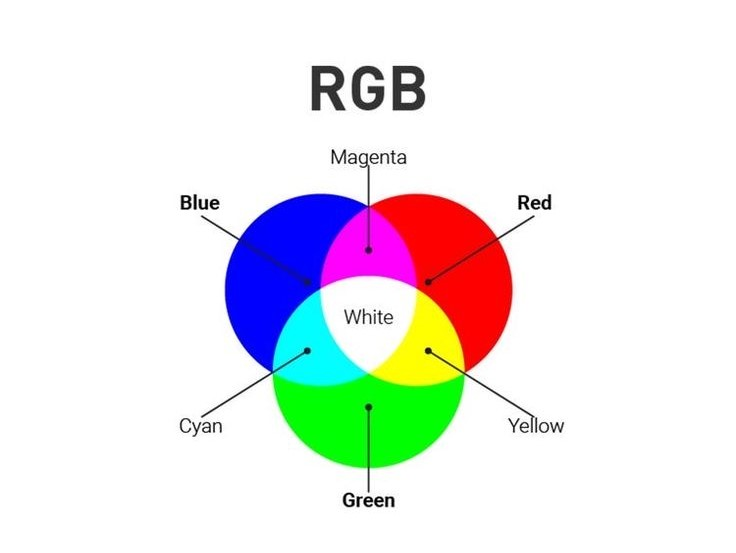
\includegraphics[width=0.5\textwidth]{figure/chapter-2-RGB.jpeg}
	\caption{RGB}
	\label{fig:2.RGB}
\end{figure}

Model warna RGB adalah salah satu model warna yang paling umum digunakan dalam citra digital. Model ini menggunakan tiga komponen warna dasar, yaitu merah (Red), hijau (Green), dan biru (Blue), untuk membentuk berbagai warna lainnya. Setiap komponen memiliki rentang nilai dari 0 hingga 255, sehingga kombinasi ketiga komponen ini dapat menghasilkan lebih dari 16 juta warna yang berbeda \cite{himmah2020identifikasi}.

Model RGB bekerja berdasarkan prinsip aditif, di mana warna-warna dihasilkan dengan menjumlahkan intensitas dari ketiga komponen tersebut. Misalnya, jika semua komponen memiliki nilai maksimum (255), maka warna yang dihasilkan adalah putih. Sebaliknya, jika semua komponen memiliki nilai minimum (0), maka warna yang dihasilkan adalah hitam. Kombinasi berbagai nilai dari ketiga komponen ini memungkinkan representasi warna yang sangat kaya dan beragam \cite{fitriyah2021dasar}.

Model RGB banyak digunakan dalam berbagai aplikasi, seperti fotografi digital, desain grafis, dan pemrosesan citra. Dalam konteks penelitian ini, model RGB digunakan untuk menganalisis citra daun bibit kelapa sawit guna mendeteksi penyakit yang mungkin terjadi. Dengan memanfaatkan informasi warna yang terkandung dalam citra, algoritma klasifikasi dapat mengidentifikasi pola-pola yang menunjukkan adanya penyakit pada daun \cite{nurhadi2024sistem}.

\subsubsection{\textit{Grayscale}} \label{II.Grayscale}
\begin{figure}[H]
	\centering
	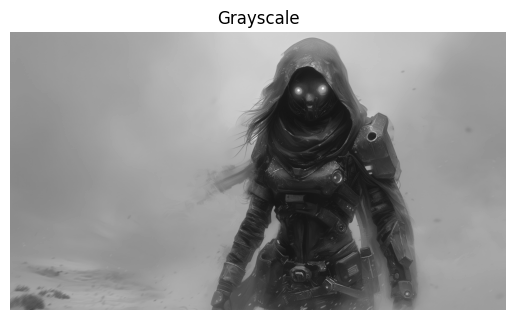
\includegraphics[width=0.5\textwidth]{figure/chapter-2-Grayscale.png}
	\caption{Grayscale}
	\label{fig:2.Grayscale}
\end{figure}

Model warna grayscale adalah representasi citra dalam skala keabuan, di mana setiap piksel hanya memiliki satu nilai intensitas yang merepresentasikan kecerahan dari hitam (0) hingga putih (255). Model ini menghilangkan informasi warna dan hanya mempertahankan informasi tentang intensitas cahaya \cite{marpaung2022computer}.

Citra grayscale sering digunakan dalam pemrosesan citra karena lebih sederhana dan lebih mudah untuk dianalisis dibandingkan dengan citra berwarna. Dalam banyak aplikasi, seperti deteksi tepi, segmentasi, dan pengenalan pola, informasi warna tidak selalu diperlukan, sehingga konversi citra berwarna menjadi grayscale dapat mengurangi kompleksitas perhitungan \cite{marpaung2022computer}.

Rumus konversi citra RGB ke grayscale yang umum digunakan adalah sebagai berikut:

\begin{equation}
I_{gray} = 0.299 \cdot R + 0.587 \cdot G + 0.114 \cdot B
\label{eq:grayscale}
\end{equation}
\myequations{Nilai Grayscale}

\noindent
dengan keterangan sebagai berikut:\\[0.5em]
\hspace*{1.5em}$I_{gray}$ : nilai intensitas piksel pada citra grayscale\\
\hspace*{1.5em}$R$ : nilai intensitas komponen merah (Red) pada piksel\\
\hspace*{1.5em}$G$ : nilai intensitas komponen hijau (Green) pada piksel\\
\hspace*{1.5em}$B$ : nilai intensitas komponen biru (Blue) pada piksel

Rumus ini menggunakan pembobotan berdasarkan sensitivitas mata manusia terhadap warna, sehingga menghasilkan representasi keabuan yang lebih natural.

% -----------------
\subsection{Identifikasi} \label{II.Identifikasi}
Identifikasi adalah proses pengenalan dan penentuan karakteristik atau atribut tertentu dari objek atau fenomena yang diamati. Dalam konteks penelitian ini, identifikasi dilakukan untuk mendeteksi dan mengklasifikasikan penyakit pada daun bibit kelapa sawit berdasarkan citra digital yang diambil dari tanaman. Proses identifikasi melibatkan beberapa langkah, seperti pra-pemrosesan citra, ekstraksi fitur, dan klasifikasi menggunakan algoritma \textit{Naïve Bayes} yang telah dioptimalkan dengan \textit{Genetic Algorithm} dan \textit{Particle Swarm Optimization} \cite{burhanuddin2024klasifikasi}.

Proses identifikasi bertujuan untuk meningkatkan akurasi dan efisiensi dalam mendeteksi penyakit pada daun bibit kelapa sawit, sehingga dapat membantu petani dalam pengambilan keputusan yang lebih baik terkait perawatan tanaman.

% -----------------
\subsection{Penyakit} \label{II.Penyakit}
Penyakit adalah kondisi abnormal yang terjadi pada organisme, baik itu manusia, hewan, maupun tumbuhan, yang disebabkan oleh berbagai faktor seperti infeksi patogen (virus, bakteri, jamur), gangguan genetik, atau faktor lingkungan. Penyakit dapat mempengaruhi fungsi normal organisme dan menyebabkan gejala klinis yang beragam \cite{pribadi2022deteksi}.

Dalam konteks penelitian ini, penyakit yang diteliti adalah penyakit pada daun bibit kelapa sawit, yang dapat mengganggu pertumbuhan dan produktivitas tanaman. Penyakit ini dapat disebabkan oleh infeksi jamur, virus, atau faktor lingkungan yang tidak optimal. Deteksi dini dan akurat terhadap penyakit pada daun bibit kelapa sawit sangat penting untuk menjaga kesehatan tanaman dan meningkatkan hasil panen.

Penyakit pada daun bibit kelapa sawit dapat menyebabkan kerugian ekonomi yang signifikan bagi petani dan industri kelapa sawit secara keseluruhan. Oleh karena itu, penelitian ini bertujuan untuk mengembangkan sistem identifikasi penyakit pada daun bibit kelapa sawit menggunakan algoritma \textit{Naïve Bayes} yang dioptimalkan dengan \textit{Genetic Algorithm} dan \textit{Particle Swarm Optimization} untuk meningkatkan akurasi dan efisiensi dalam mendeteksi penyakit tersebut \cite{pribadi2022deteksi}.

% -----------------
\subsection{Ekstraksi Fitur} \label{II.Ekstraksi Fitur}
Ekstraksi fitur adalah proses pengambilan informasi penting dari citra yang dapat digunakan untuk membedakan antara kelas-kelas yang berbeda. Dalam konteks penelitian ini, ekstraksi fitur dilakukan untuk mendapatkan karakteristik yang relevan dari citra daun bibit kelapa sawit yang terinfeksi penyakit. Fitur-fitur ini akan digunakan sebagai input untuk algoritma klasifikasi \textit{Naïve Bayes} yang telah dioptimalkan dengan \textit{Genetic Algorithm} dan \textit{Particle Swarm Optimization} \cite{alwy2023klasifikasi}.

Ekstraksi fitur dapat dilakukan dengan berbagai metode, seperti analisis tekstur, warna, bentuk, dan pola. Dalam penelitian ini, fitur yang diekstraksi meliputi informasi warna (RGB), tekstur (menggunakan metode Gray Level Co-occurrence Matrix/GLCM), dan bentuk daun. Fitur-fitur ini diharapkan dapat memberikan informasi yang cukup untuk membedakan antara daun bibit kelapa sawit yang sehat dan yang terinfeksi penyakit.

\subsubsection{Ekstraksi Fitur Warna} \label{II.Ekstraksi Fitur Warna}
Ekstraksi fitur warna adalah proses pengambilan informasi warna dari citra yang dapat digunakan untuk membedakan antara kelas-kelas yang berbeda. Dalam penelitian ini, fitur warna diekstraksi dari citra daun bibit kelapa sawit yang terinfeksi penyakit menggunakan model warna RGB. Fitur warna yang diekstraksi meliputi nilai rata-rata, deviasi standar, dan histogram dari setiap komponen warna (merah, hijau, dan biru) \cite{yohannes2023klasifikasi}.

Rumus ekstraksi fitur warna RGB secara matematis dapat dinyatakan sebagai berikut:
\begin{equation}
	\overline{C} = \frac{1}{N} \sum_{i=1}^{N} C_i \label{eq:mean-color}
\end{equation}
\myequations{Rata-rata fitur warna C}
\begin{equation}
	\sigma_C = \sqrt{ \frac{1}{N} \sum_{i=1}^{N} (C_i - \overline{C})^2 } \label{eq:std-color}
\end{equation}
\myequations{Standar deviasi fitur warna C}


\noindent
dengan $C$ mewakili salah satu komponen warna (R, G, atau B), $\overline{C}$ adalah nilai rata-rata, $\sigma_C$ adalah deviasi standar, dan $N$ adalah jumlah piksel pada citra. Rumus ini digunakan untuk memperoleh karakteristik statistik warna yang dapat membedakan kondisi daun sehat dan terinfeksi penyakit.

Untuk normalisasi warna RGB, digunakan rumus:
\begin{equation}
	R = \frac{r}{r+g+b} \label{eq:norm-r}
\end{equation}
\myequations{Normalisasi komponen R}
\begin{equation}
	G = \frac{g}{r+g+b} \label{eq:norm-g}
\end{equation}
\myequations{Normalisasi komponen G}
\begin{equation}
	B = \frac{b}{r+g+b} \label{eq:norm-b}
\end{equation}
\myequations{Normalisasi komponen B}
\noindent

dengan $r$, $g$, dan $b$ mewakili nilai intensitas komponen warna merah, hijau, dan biru pada piksel, sedangkan $R$, $G$, dan $B$ adalah nilai yang sudah dinormalisasi.

Histogram warna memberikan informasi tentang distribusi intensitas warna dalam citra, yang dapat digunakan untuk membedakan antara daun bibit kelapa sawit yang sehat dan yang terinfeksi penyakit. Histogram warna dihitung dengan menghitung jumlah piksel pada setiap rentang intensitas warna (0-255) untuk setiap komponen warna.

\subsubsection{Ekstraksi Fitur Tekstur} \label{II.Ekstraksi Fitur Tektur}
Ekstraksi fitur tekstur adalah proses pengambilan informasi tentang pola dan struktur permukaan dari citra. Dalam penelitian ini, fitur tekstur diekstraksi menggunakan metode \textit{Gray Level Co-occurrence Matrix (GLCM)}. GLCM adalah matriks yang menggambarkan frekuensi kemunculan pasangan piksel dengan nilai intensitas tertentu pada jarak dan arah tertentu \cite{sinaga2024klasifikasi}.

GLCM dapat digunakan untuk menghitung berbagai fitur tekstur, seperti kontras, energi, homogenitas, dan entropi. Fitur-fitur ini dapat memberikan informasi yang berguna untuk membedakan antara daun bibit kelapa sawit yang sehat dan yang terinfeksi penyakit.

\begin{figure}[H]
	\centering
	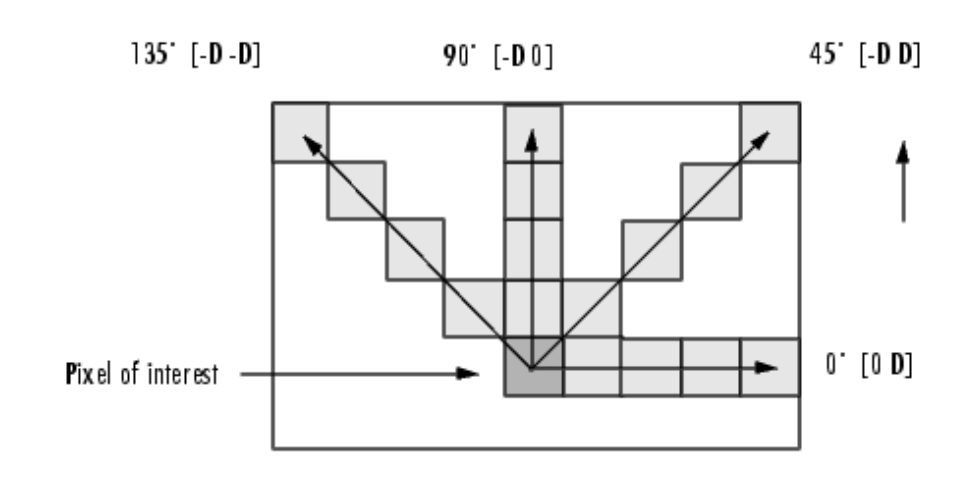
\includegraphics[width=0.5\textwidth]{figure/chapter-2-GLCM.png}
	\caption{\textit{Gray Level Co-occurrence Matrix (GLCM)}}
	\label{fig:2.GLCM}
\end{figure}

Rumus GLCM untuk menghitung frekuensi kemunculan pasangan piksel dapat dinyatakan sebagai berikut:
\begin{equation}
	P(i,j) = \sum_{x,y} \delta(I(x,y), i) \cdot \delta(I(x+dx,y+dy), j)
	\label{eq:glcm}
\end{equation}
\myequations{Nilai GLCM}
\noindent

dengan $P(i,j)$ adalah nilai GLCM untuk pasangan piksel dengan intensitas $i$ dan $j$, $I(x,y)$ adalah nilai intensitas piksel pada posisi $(x,y)$, dan $\delta$ adalah fungsi delta Kronecker yang bernilai 1 jika argumennya sama dan 0 jika berbeda. Parameter $dx$ dan $dy$ menentukan jarak dan arah antara pasangan piksel yang dihitung.

Fitur tekstur yang umum dihitung dari GLCM, meliputi Contrast (Kontras), Correlation (Korelasi), Energy (Energi/Uniformity/ASM), dan Homogeneity (Homogenitas) \cite{hanafi2025analisis}.
\begin{enumerate}
	\item \textbf{Contrast (Kontras)} \label{II.Ekstraksi Fitur Tekstur.Kontras}
\end{enumerate}

Kontras merupakan fitur GLCM yang digunakan untuk mengukur perbedaan lokal dalam citra. Nilai kontras yang tinggi menunjukkan variasi intensitas yang besar antara piksel bersebelahan.
\begin{equation}
	\text{Contrast} = \sum_{i=0}^{N_g-1} \sum_{j=0}^{N_g-1} (i-j)^2 \, P(i,j)
	\label{eq:glcm-contrast}
\end{equation}
\myequations{Nilai Kontras}

\begin{enumerate} [resume]
	\item \textbf{Correlation (Korelasi)} \label{II.Ekstraksi Fitur Tekstur.Korelasi}
\end{enumerate}
Korelasi adalah fitur GLCM yang digunakan untuk mengukur hubungan linear antara nilai intensitas piksel pada pasangan piksel dalam matriks. Nilai korelasi mencerminkan seberapa jauh hubungan antara baris dan kolom dalam GLCM, semakin tinggi nilai korelasi, semakin kuat hubungan antara intensitas piksel yang bersebelahan. Hubungan ini dapat dihitung menggunakan rumus berikut:
\begin{equation}
	\text{Correlation} = \frac{\sum_{i=0}^{N_g-1} \sum_{j=0}^{N_g-1} (i-\mu_i)(j-\mu_j) P(i,j)}{\sigma_i \sigma_j}
	\label{eq:glcm-correlation}
\end{equation}
\myequations{Nilai Korelasi}

dengan $\mu_i$, $\mu_j$ adalah nilai rata-rata baris dan kolom, serta $\sigma_i$, $\sigma_j$ merupakan simpangan baku (standar deviasi) dari baris dan kolom.
\begin{enumerate}[resume]
	\item \textbf{Energy (Energi/Uniformity/ASM)} \label{II.Ekstraksi Fitur Tekstur.Energi}
\end{enumerate}

Energy mengukur tingkat keseragaman tekstur dalam citra. Semakin seragam sebuah citra, semakin tinggi nilai energinya.

\begin{equation}
\text{Energy} = \sum_{i=0}^{N_g-1} \sum_{j=0}^{N_g-1} P(i,j)^2
\label{eq:glcm-energy}
\end{equation}
\myequations{Nilai Energi}

\begin{enumerate}[resume]
	\item \textbf{Homogeneity (Homogenitas)} \label{II.Ekstraksi Fitur Tekstur.Energi}
\end{enumerate}

Homogenitas mengukur kedekatan nilai elemen dalam GLCM terhadap diagonal utama. Nilai homogenitas tinggi menunjukkan bahwa nilai elemen lebih terkonsentrasi di sekitar diagonal.
\begin{equation}
\text{Homogeneity} = \sum_{i=0}^{N_g-1} \sum_{j=0}^{N_g-1} \frac{P(i,j)}{1 + |i-j|}
\label{eq:glcm-homogeneity}
\end{equation}
\myequations{Nilai Homogenitas}


% -----------------
\subsection{Machine Learning} \label{II. Machine Learning}
Machine Learning adalah cabang dari kecerdasan buatan (Artificial Intelligence) yang berfokus pada pengembangan algoritma dan model yang memungkinkan komputer untuk belajar dari data dan membuat prediksi atau keputusan tanpa perlu diprogram secara eksplisit. Machine Learning mengandalkan teknik statistik dan matematis untuk menganalisis pola dalam data, sehingga dapat digunakan untuk berbagai aplikasi, seperti klasifikasi, regresi, clustering, dan rekomendasi \cite{diana2023penggunaan}.

\begin{figure}[H]
	\centering
	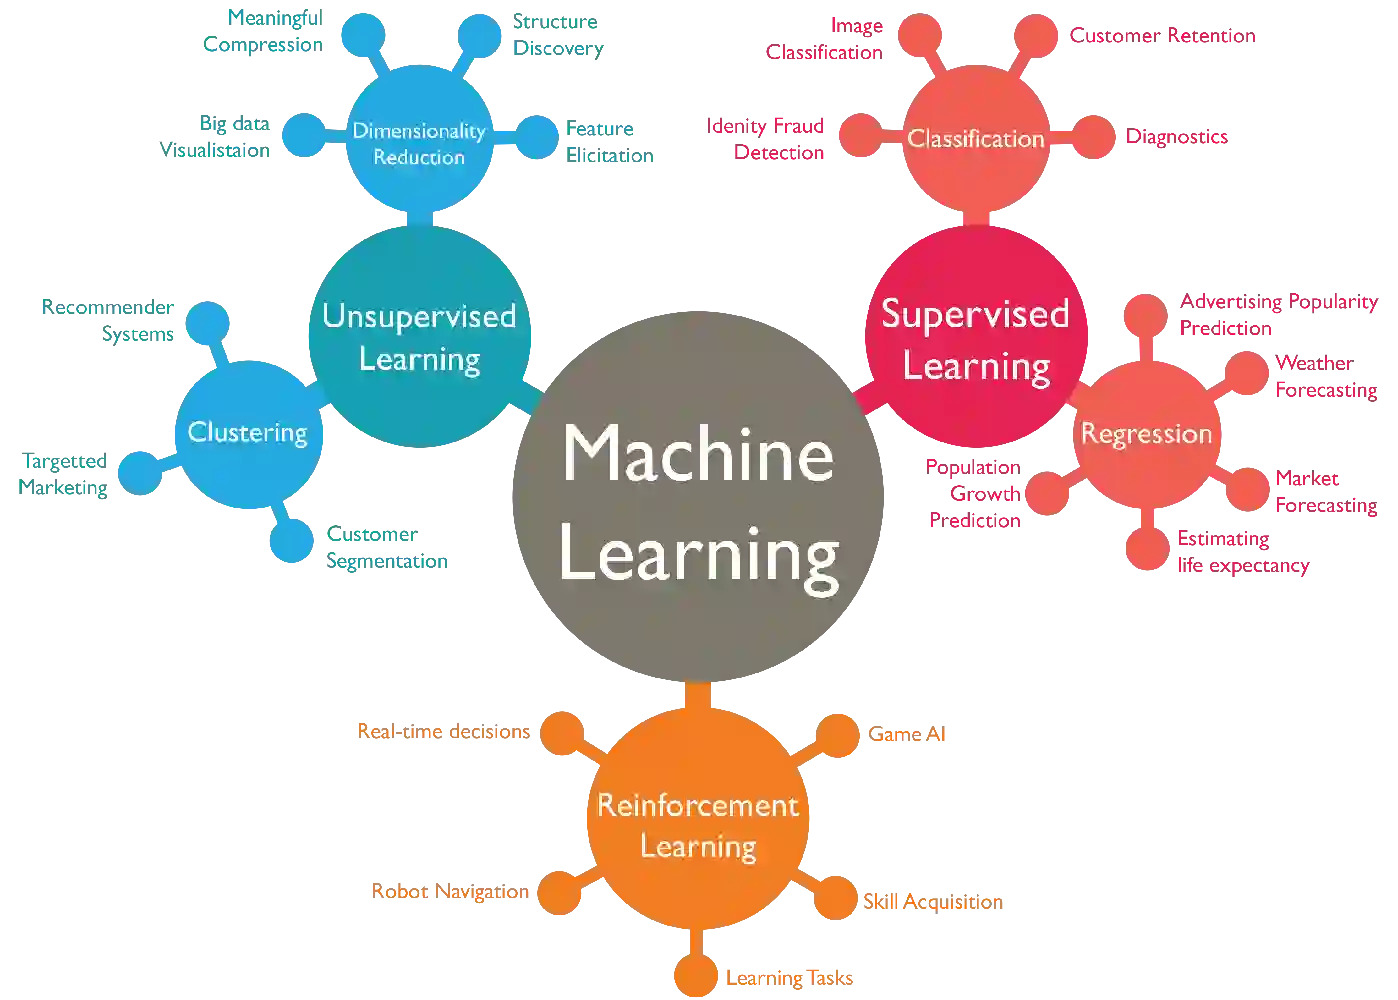
\includegraphics[width=0.5\textwidth]{figure/chapter-2-machine-learning.png}
	\caption{Machine Learning}
	\label{fig:2. Machine Learning}
\end{figure}

Dalam konteks penelitian ini, Machine Learning digunakan untuk mengembangkan sistem identifikasi penyakit pada daun bibit kelapa sawit. Algoritma yang digunakan adalah \textit{Naïve Bayes} yang dioptimalkan dengan \textit{Genetic Algorithm} dan \textit{Particle Swarm Optimization}. Dengan menggunakan teknik Machine Learning, sistem dapat belajar dari data citra daun bibit kelapa sawit yang terinfeksi penyakit dan mengklasifikasikan kondisi daun berdasarkan fitur-fitur yang diekstraksi.

% % -----------------
% \subsection{Deep Learning} \label{II. Deep Learning}
% Deep Learning adalah subbidang dari Machine Learning yang menggunakan jaringan saraf tiruan (neural networks) dengan banyak lapisan (deep neural networks) untuk mempelajari representasi data yang kompleks. Deep Learning telah terbukti sangat efektif dalam berbagai aplikasi, seperti pengenalan citra, pemrosesan bahasa alami, dan permainan komputer.

% \begin{figure}[H]
% 	\centering
% 	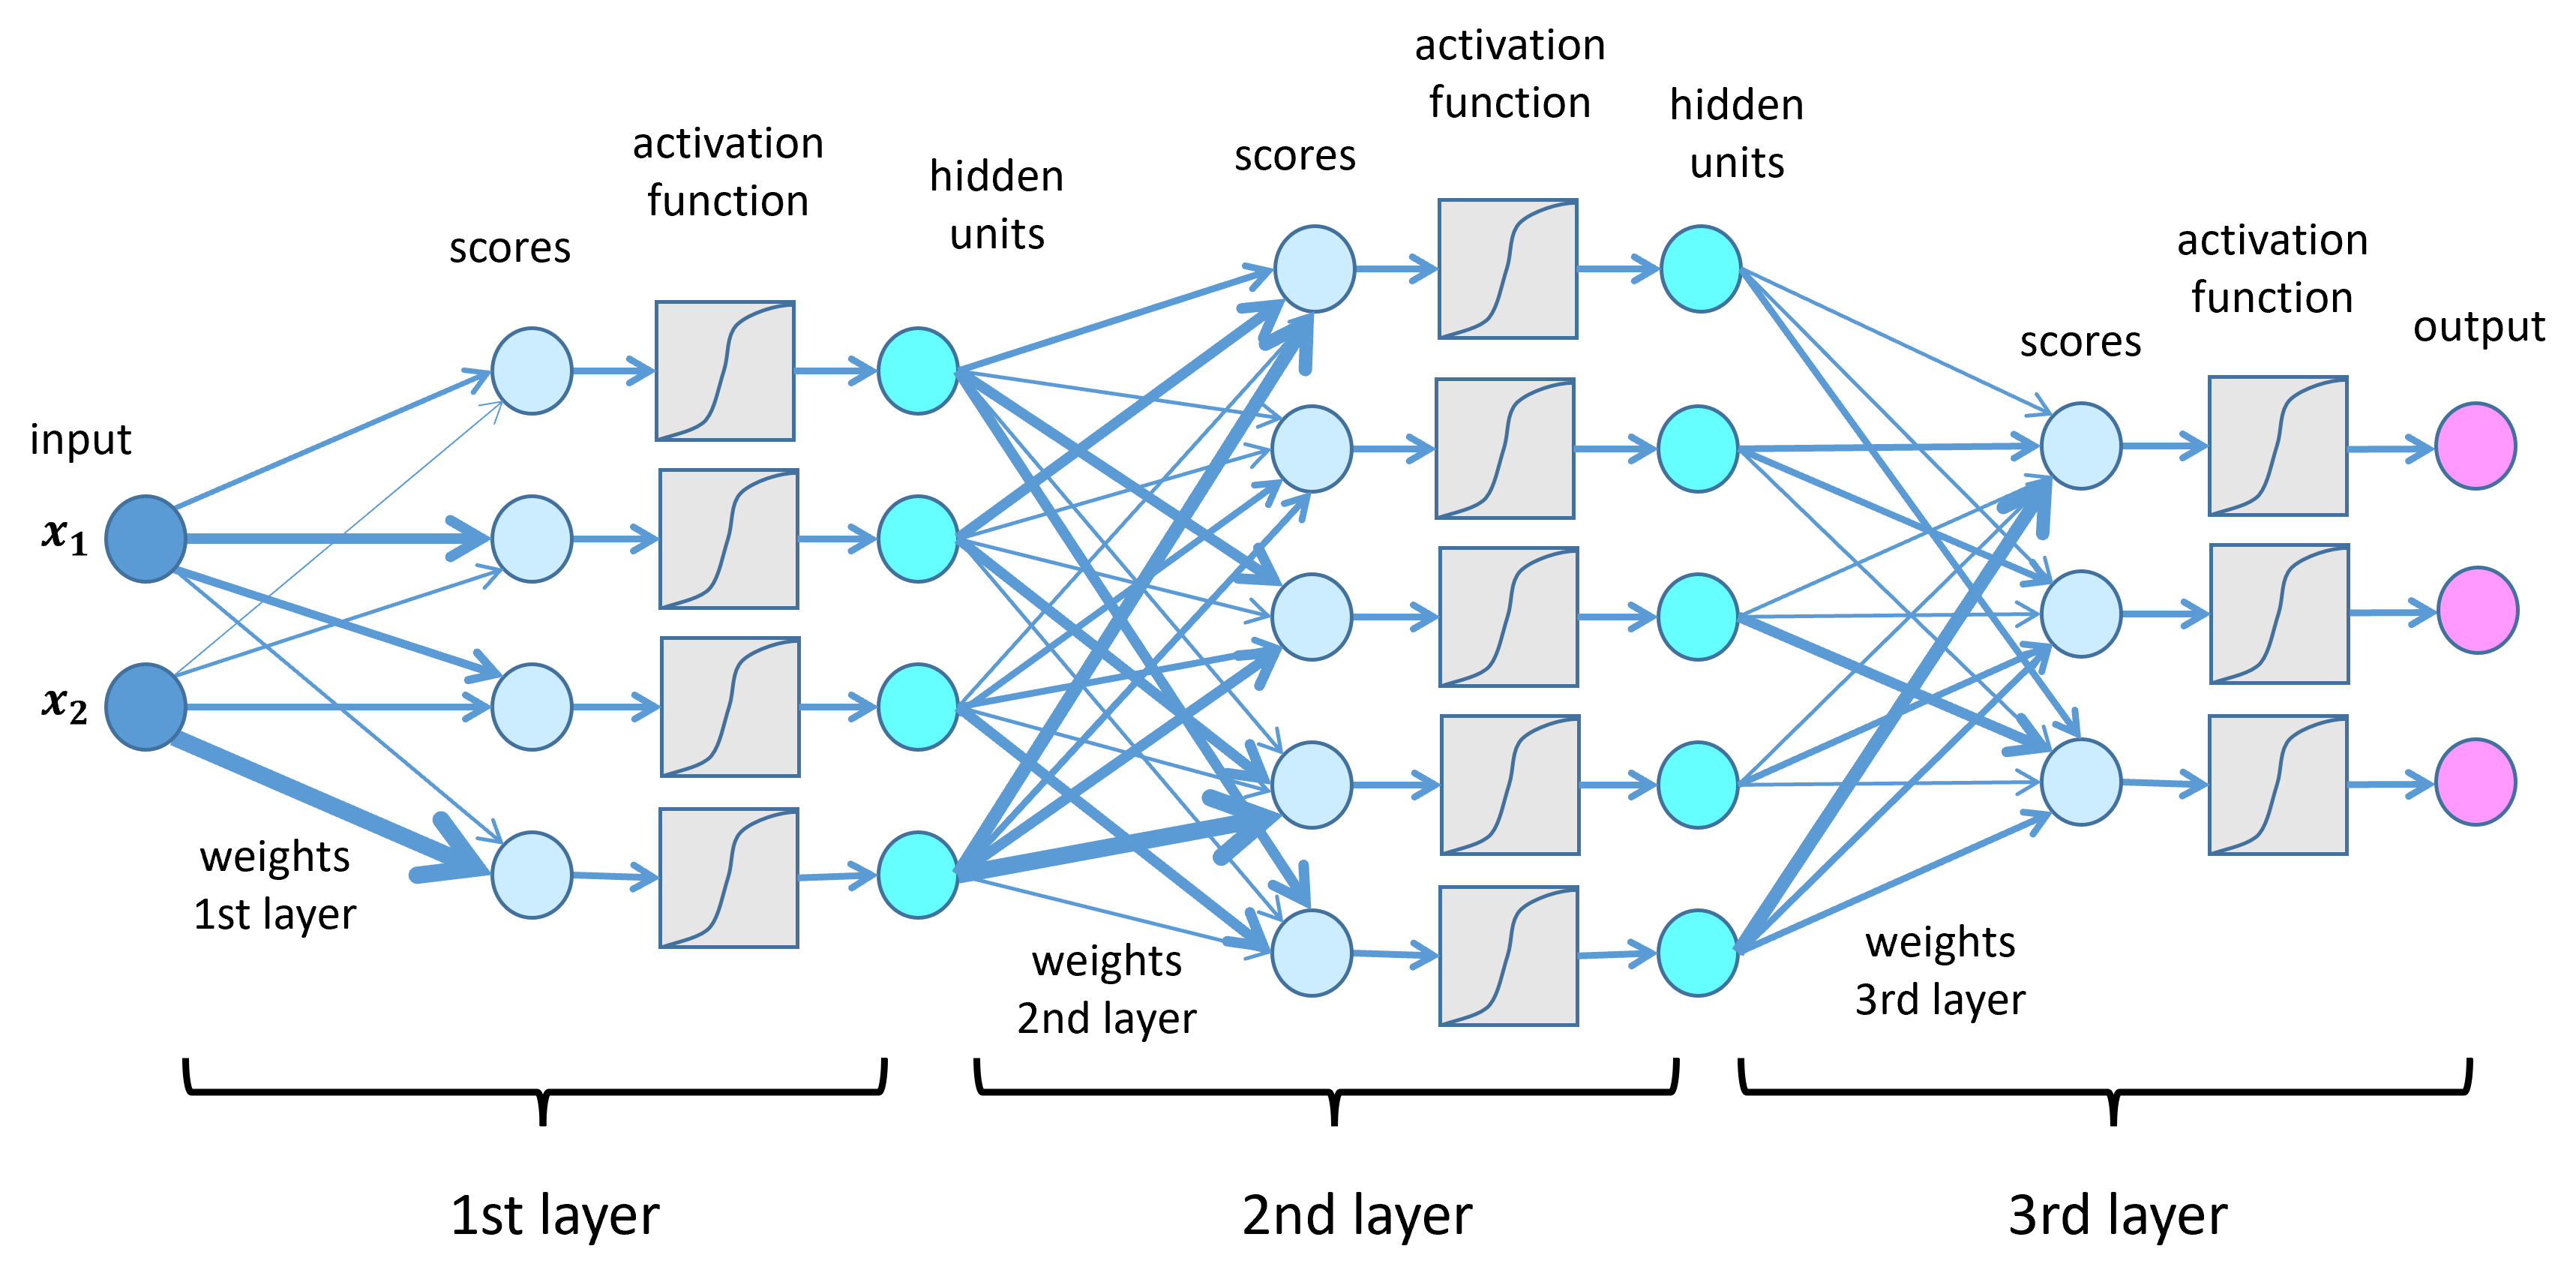
\includegraphics[width=0.5\textwidth]{figure/chapter-2-deep-learning.png}
% 	\caption{Deep Learning}
% 	\label{fig:2. Deep Learning}
% \end{figure}

% Deep Learning menggunakan arsitektur jaringan saraf yang terdiri dari beberapa lapisan, di mana setiap lapisan belajar untuk mengekstraksi fitur yang semakin kompleks dari data input. Proses pembelajaran dilakukan melalui propagasi maju (forward propagation) dan pembaruan bobot (weight update) menggunakan algoritma backpropagation. Dengan menggunakan teknik ini, Deep Learning dapat mengidentifikasi pola-pola yang sulit dikenali oleh metode tradisional.

% Deep Learning bekerja dengan cara mengolah data melalui beberapa lapisan neuron yang saling terhubung, di mana setiap lapisan belajar untuk mengekstraksi fitur yang semakin kompleks dari data input. Proses ini dilakukan secara otomatis tanpa memerlukan fitur yang diekstraksi secara manual, sehingga memungkinkan model untuk belajar dari data mentah.

% -----------------
\subsection{Segmentasi Citra} \label{II. Segmentasi Citra}
Segmentasi citra adalah proses pemisahan citra menjadi beberapa bagian atau objek yang lebih kecil untuk memudahkan analisis dan pengolahan. Dalam konteks penelitian ini, segmentasi citra digunakan untuk mengidentifikasi dan mengekstraksi area daun bibit kelapa sawit yang terinfeksi penyakit dari latar belakang citra \cite{wijayaimplementasi}.

Segmentasi citra dapat dilakukan dengan berbagai metode, seperti thresholding, region growing, clustering, dan deteksi tepi. Metode yang dipilih tergantung pada karakteristik citra dan tujuan analisis. Dalam penelitian ini, metode segmentasi yang digunakan adalah thresholding untuk memisahkan area daun dari latar belakang berdasarkan nilai intensitas warna.

Selain thresholding, penelitian ini juga memanfaatkan \textit{Photoroom}, yaitu website untuk menghilangkan latar belakang pada citra. Dengan \textit{Photoroom}, proses segmentasi menjadi lebih efisien dan akurat, terutama untuk citra dengan latar belakang yang kompleks. Penggunaan \textit{Photoroom} memungkinkan area daun dapat diekstraksi secara otomatis tanpa perlu pengaturan threshold manual, sehingga mempercepat proses pra-pemrosesan citra \cite{wijayaimplementasi}.

Setelah proses segmentasi, area daun yang terinfeksi penyakit dapat dianalisis lebih lanjut untuk ekstraksi fitur dan klasifikasi menggunakan algoritma \textit{Naïve Bayes} yang telah dioptimalkan dengan \textit{Genetic Algorithm} dan \textit{Particle Swarm Optimization}. 

% -----------------
\subsection{Hyperparameter} \label{II. Hyperparameter}
Hyperparameter adalah parameter yang ditentukan sebelum proses pelatihan model dimulai dan tidak diperoleh dari data pelatihan. Hyperparameter berfungsi untuk mengontrol proses pembelajaran dan mempengaruhi kinerja model. Dalam konteks penelitian ini, hyperparameter digunakan untuk mengoptimalkan algoritma \textit{Naïve Bayes} yang diterapkan pada citra daun bibit kelapa sawit \cite{burhanuddin2024klasifikasi}.

Pemilihan hyperparameter yang tepat sangat penting untuk mencapai kinerja model yang optimal. Dalam penelitian ini, hyperparameter dioptimalkan menggunakan algoritma \textit{Genetic Algorithm} dan \textit{Particle Swarm Optimization} untuk meningkatkan akurasi klasifikasi penyakit pada daun bibit kelapa sawit \cite{vratiwi2024penerapan}.

Pada penelitian ini, hyperparameter yang digunakan adalah \textit{Variable Smoothing}. \textit{Variable Smoothing} adalah teknik yang digunakan untuk menghindari pembagian dengan nol pada perhitungan probabilitas dalam algoritma \textit{Naïve Bayes}. Dengan menggunakan \textit{Variable Smoothing}, setiap frekuensi kata dalam perhitungan probabilitas akan ditambahkan dengan nilai \textit{Smoothing} yang ditentukan. Hal ini membantu meningkatkan stabilitas dan akurasi model klasifikasi. 

% -----------------
\subsection{Confusion Matrix} \label{II. ConfusionMatrix}
\textit{Confusion Matrix} adalah alat evaluasi yang digunakan untuk mengukur kinerja model klasifikasi dengan membandingkan hasil prediksi model dengan label sebenarnya. \textit{Confusion Matrix} memberikan informasi tentang jumlah prediksi yang benar dan salah untuk setiap kelas dalam dataset \cite{rijal2024deteksi}.

\textit{Confusion Matrix} dapat digunakan untuk menghitung berbagai metrik evaluasi, seperti akurasi, presisi, recall, dan F1-score. Metrik-metrik ini memberikan gambaran yang lebih jelas tentang kinerja model klasifikasi dalam mendeteksi penyakit pada daun bibit kelapa sawit.

\begin{figure}[H]
	\centering
	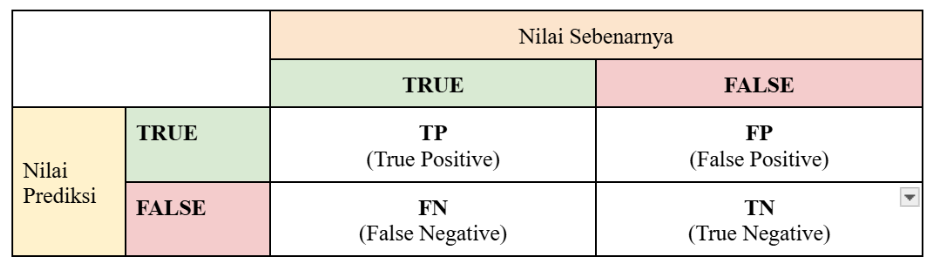
\includegraphics[width=1\textwidth]{figure/chapter-2-Confusion-Matrix.png}
	\caption{Confusion Matrix}
	\label{fig:2.ConfusionMatrix}
\end{figure}
Dengan keterangan sebagai berikut:\\[0.5em]
\hspace*{2em}$TP$ : jumlah data yang sebenarnya positif dan diprediksi positif\\
\hspace*{2em}$FP$ : jumlah data yang sebenarnya negatif tetapi diprediksi positif\\
\hspace*{2em}$FN$ : jumlah data yang sebenarnya positif tetapi diprediksi negatif\\
\hspace*{2em}$TN$ : jumlah data yang sebenarnya negatif dan diprediksi negatif

Dari Confusion Matrix di atas, nilai-nilai tersebut digunakan untuk menghitung metrik evaluasi sebagai berikut.


\begin{enumerate}
	\item {Akurasi (Accuracy)}\label{II.Ekstraksi Fitur Tekstur.Kontras}
\end{enumerate}
Akurasi (\textit{Accuracy}) menunjukkan seberapa akurat prediksi yang benar dari metode yang digunakan:
\begin{equation}
    accuracy = \frac{TP + TN}{TP + FP + TN + FN}
    \label{eq:accuracy}
\end{equation}
\myequations{Nilai Akurasi}

\begin{enumerate} [resume]
	\item {Presisi (Precision)}\label{II.Ekstraksi Fitur Tekstur.Kontras}
\end{enumerate}
Presisi (\textit{Precision}) adalah rasio antara jumlah prediksi positif yang benar (TP) dengan keseluruhan hasil prediksi positif (TP + FP), yang menggambarkan tingkat keakuratan prediksi positif dari model:
\begin{equation}
    precision = \frac{TP}{TP + FP}
    \label{eq:precision}
\end{equation}
\myequations{Nilai Presisi}
\\
\begin{enumerate}  [resume]
	\item {Recall}\label{II.Ekstraksi Fitur Tekstur.Kontras}
\end{enumerate}
Recall adalah rasio antara jumlah prediksi positif yang benar (TP) dengan jumlah keseluruhan data yang sebenarnya positif (TP + FN), yang menunjukkan kemampuan model dalam menemukan data positif yang sebenarnya:
\begin{equation}
    recall = \frac{TP}{TP + FN}
    \label{eq:recall}
\end{equation}
\myequations{Nilai Recall}

% -----------------
\subsection{Roboflow} \label{II.Roboflow}
Roboflow adalah platform yang menyediakan alat dan layanan untuk membantu pengembang dan peneliti dalam membangun, melatih, dan menerapkan model pembelajaran mesin untuk pengenalan citra. Roboflow menawarkan berbagai fitur, termasuk pengumpulan data, anotasi, augmentasi, dan pelatihan model \cite{saepudin2024analisis}.

Dengan Roboflow, pengguna dapat dengan mudah mengunggah citra, menandai objek dalam citra, dan melakukan augmentasi data untuk meningkatkan variasi dan jumlah data pelatihan. Platform ini juga menyediakan integrasi dengan berbagai framework pembelajaran mesin populer, seperti TensorFlow, PyTorch, dan Keras.

Roboflow memungkinkan pengguna untuk membangun model pembelajaran mesin tanpa perlu memiliki pengetahuan mendalam tentang pemrograman atau algoritma pembelajaran mesin. Dengan antarmuka yang intuitif dan alat yang mudah digunakan, Roboflow membantu mempercepat proses pengembangan model pengenalan citra.

Roboflow juga menyediakan API dan SDK yang memungkinkan pengguna untuk mengintegrasikan model yang telah dilatih ke dalam aplikasi mereka. Dengan menggunakan Roboflow, pengguna dapat dengan cepat membangun dan menerapkan model pembelajaran mesin untuk berbagai aplikasi, seperti deteksi objek, segmentasi citra, dan klasifikasi citra.

Roboflow juga menyediakan fitur untuk mengelola dan menyimpan dataset, serta melakukan kolaborasi dengan tim dalam proyek pembelajaran mesin. Dengan semua fitur ini, Roboflow menjadi alat yang sangat berguna bagi pengembang dan peneliti yang ingin membangun model pembelajaran mesin untuk pengenalan citra dengan cepat dan efisien.

% -----------------
\subsection{StreamLit} \label{II.StreamLit}
Streamlit adalah framework open-source yang digunakan untuk membangun aplikasi web interaktif dengan cepat dan mudah, khususnya untuk aplikasi yang berkaitan dengan data sains dan pembelajaran mesin. Dengan Streamlit, pengguna dapat membuat antarmuka pengguna (UI) yang menarik dan responsif tanpa perlu memiliki pengetahuan mendalam tentang pengembangan web.
Streamlit memungkinkan pengguna untuk menulis aplikasi web menggunakan bahasa pemrograman Python, sehingga memudahkan integrasi dengan berbagai pustaka dan alat analisis data yang sudah ada \cite{wahyuni2024transformasi}.

Dengan menggunakan Streamlit, pengguna dapat dengan cepat membangun aplikasi web yang menarik dan interaktif untuk memvisualisasikan data, menjalankan model pembelajaran mesin, dan berbagi hasil analisis dengan orang lain. Dalam konteks penelitian ini, Streamlit digunakan untuk membuat antarmuka pengguna yang memungkinkan pengguna untuk mengunggah citra daun bibit kelapa sawit dan mendapatkan hasil klasifikasi penyakit secara real-time.
% -----------------